\section{Mô hình hoá hệ thống (System modelling)}

%%%%% Use case diagram
\subsection{Lược đồ Use-Case}


\subsubsection{Use Case cho Người Dùng - OLD}
\begin{figure}[H]
    \centering
    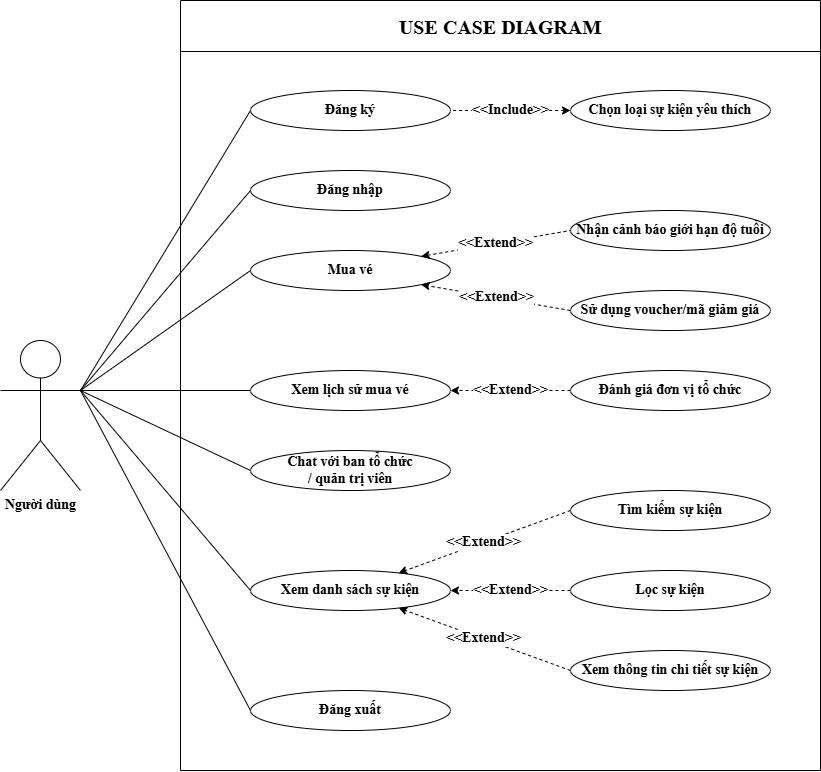
\includegraphics[width=1\textwidth]{Images/User_UseCaseDiagram.png}
    \vspace{10pt}
    \caption{Use Case Diagram -- Người dùng}
    \label{fig:uc_user}
\end{figure}

\subsubsubsection{Xem, tìm kiếm và lọc thông tin sự kiện}
\begin{table}[H]
\centering
\renewcommand{\arraystretch}{1.3}
\setlength{\tabcolsep}{8pt}
\begin{tabularx}{\textwidth}{|l|X|}
\hline
\textbf{Tên Use Case} & Tìm kiếm và xem thông tin sự kiện \\ \hline
\textbf{Tác nhân} & Người dùng \\ \hline
\textbf{Mục đích} & Giúp người dùng tìm sự kiện theo từ khóa, lọc theo các tiêu chí, xem thông tin chi tiết của sự kiện. \\ \hline
\textbf{Tiền điều kiện} & Không có \\ \hline
\textbf{Hậu điều kiện} & Chi tiết sự kiện phù hợp được hiển thị. \\ \hline
\textbf{Mô tả ngắn gọn} & Người dùng nhập từ khóa và có thể áp dụng bộ lọc (Địa điểm, Ngày diễn ra sự kiện, Giá vé tối thiểu) để tìm kiếm sự kiện; hệ thống trả về kết quả phù hợp, người dùng chọn sự kiện quan tâm để xem chi tiết. \\ \hline
\textbf{Luồng chính} &
1. Người dùng nhập từ khóa vào thanh tìm kiếm trên trang chủ hoặc trang sự kiện. \newline
2. Nếu áp dụng bộ lọc, người dùng có thể lọc theo các tiêu chí: \newline
\hspace*{1em}a) Địa điểm: Thành phố hoặc tỉnh diễn ra sự kiện \newline
\hspace*{1em}b) Ngày diễn ra sự kiện: Những sự kiện có ngày bắt đầu tổ chức nằm trong phạm vi ngày tháng được chọn \newline
\hspace*{1em}d) Giá vé tối thiểu: Giá hạng vé thấp nhất của sự kiện \newline
3. Hệ thống thực hiện truy vấn cơ sở dữ liệu, tìm kiếm sự kiện phù hợp. \newline
4. Hệ thống hiển thị danh sách sự kiện (gồm Poster, Tên, Thời gian, Địa điểm, Giá tối thiểu) theo thứ tự liên quan. \newline
5. Người dùng nhấp vào sự kiện để xem chi tiết. \newline
6. Hệ thống hiển thị: Tên, Poster, địa điểm, ngày tổ chức, mô tả sự kiện, sơ đồ chỗ ngồi hoặc vị trí các hạng vé, giá và số lượng còn lại ứng với các hạng vé hoặc vị trí ghế ngồi, nút mua vé, đơn vị tổ chức (tên, mô tả) và nút chat với Ban tố chức. \newline
7. Người dùng có thể nhấp “Mua ngay” hoặc "Chat vơi Ban tổ chức" để tiếp tục. \\ \hline
\textbf{Luồng thay thế} &
2a. Không tìm thấy kết quả: \newline
\hspace*{1em}Hệ thống hiển thị “Không tìm thấy sự kiện” và gợi ý sự kiện phổ biến hoặc sắp diễn ra. \newline
2b. Sự kiện không còn slot: \newline
\hspace*{1em}Hệ thống hiển thị “Hết vé” và vô hiệu hóa nút mua. \\ \hline
\textbf{Điều kiện lỗi} &
\textbf{Trường hợp lỗi 1:} Truy vấn cơ sở dữ liệu thất bại — Hệ thống hiển thị danh sách sự kiện phổ biến được lưu trữ. \newline
\textbf{Trường hợp lỗi 2:} Thời gian phản hồi quá 3 giây — Hệ thống thông báo “Vui lòng thử lại!”. \\ \hline
\end{tabularx}
\vspace{15pt}
\caption{Đặc tả Use Case -- Xem, tìm kiếm và lọc thông tin sự kiện}
\label{tab:uc_search_event}
\end{table}

\subsubsubsection{Truy cập chức năng yêu cầu xác thực}

\begin{table}[H]
\centering
\renewcommand{\arraystretch}{1.3}
\setlength{\tabcolsep}{8pt}
\begin{tabularx}{\textwidth}{|l|X|}
\hline
\textbf{Tên Use Case} & Truy Cập Chức Năng Yêu Cầu Xác Thực \\ \hline
\textbf{Tác nhân} & Người dùng \\ \hline
\textbf{Mục đích} & Đảm bảo người dùng đã đăng nhập thành công để truy cập các chức năng cá nhân hóa và nhạy cảm, tránh truy cập trái phép. \\ \hline
\textbf{Điều kiện tiên quyết} &
Người dùng cố gắng thực hiện một trong các chức năng sau: \newline
\hspace*{1em}- Mua vé. \newline
\hspace*{1em}- Xem lịch sử mua vé \newline
\hspace*{1em}- Chat với đơn vị tổ chức sự kiện hoặc quản trị viên. \\ \hline
\textbf{Điều kiện hậu quyết} & Các chức năng được kích hoạt nếu đăng nhập thành công; nếu không, người dùng bị chuyển hướng đến trang đăng nhập. \\ \hline
\textbf{Mô tả ngắn gọn} & Hệ thống kiểm tra trạng thái xác thực (JWT token hoặc session) trước khi cho phép truy cập các chức năng yêu cầu đăng nhập, bao gồm: mua vé, xem lịch sử mua vé và chat với đơn vị tổ chức sự kiện hoặc quản trị viên..\\ \hline
\textbf{Quy trình bình thường} &
1. Người dùng cố gắng truy cập một chức năng yêu cầu đăng nhập (ví dụ: nhấp “Mua vé” hoặc “Vé của tôi”). \newline
2. Hệ thống kiểm tra trạng thái xác thực (JWT token hợp lệ trong localStorage/session). \newline
3. Nếu đã đăng nhập thành công, hệ thống cho phép tiếp tục thực hiện chức năng tương ứng (ví dụ: chuyển đến trang mua vé hoặc hiển thị lịch sử). \newline
4. Hệ thống ghi log truy cập để theo dõi hoạt động. \\ \hline
\textbf{Quy trình thay thế} &
2a. Chưa đăng nhập hoặc token hết hạn: \newline
\hspace*{1em}- Hệ thống hiển thị modal/popup yêu cầu đăng nhập (với liên kết đến trang đăng nhập). \newline
\hspace*{1em}- Người dùng hoàn tất đăng nhập \newline
\hspace*{1em}- Sau khi đăng nhập thành công, hệ thống tự động chuyển hướng trở lại chức năng ban đầu. \\ \hline
\textbf{Điều kiện lỗi} &
- Trường hợp lỗi 1: Token không hợp lệ hoặc bị giả mạo $\rightarrow$ Hệ thống vô hiệu hóa token, ghi log bảo mật và buộc đăng nhập lại. \newline
- Trường hợp lỗi 2: Lỗi kiểm tra xác thực (kết nối backend thất bại) $\rightarrow$ Hệ thống hiển thị “Lỗi hệ thống, vui lòng thử lại” và ghi log để kiểm tra. \\ \hline
\end{tabularx}
\vspace{15pt}
\caption{Đặc tả Use Case -- Truy Cập Chức Năng Yêu Cầu Xác Thực}
\label{tab:uc_auth_access}
\end{table}

\subsubsubsection{Mua vé}

\begin{table}[H]
\centering
\renewcommand{\arraystretch}{1.3}
\setlength{\tabcolsep}{8pt}
\begin{tabularx}{\textwidth}{|l|X|}
\hline
\textbf{Tên Use Case} & Mua vé sự kiện (bao gồm cảnh báo độ tuổi và áp dụng voucher/mã giảm giá) \\ \hline
\textbf{Tác nhân} & Người dùng \\ \hline
\textbf{Mục đích} & Cho phép người dùng mua vé sự kiện an toàn qua MoMo, đồng thời áp dụng mã giảm giá hay voucher(nếu có) và nhận cảnh báo giới hạn độ tuổi trước khi thanh toán. \\ \hline
\textbf{Điều kiện tiên quyết} &
- Người dùng đã đăng nhập thành công. \newline
- Sự kiện tồn tại, còn slot vé khả dụng. \\ \hline
\textbf{Điều kiện hậu quyết} &
- Thanh toán hoàn tất, vé được cấp thành công. \newline
- Lịch sử mua vé được cập nhật. \\ \hline
\textbf{Mô tả ngắn gọn} &
Người dùng chọn hạng vé, nhận cảnh báo độ tuổi (nếu có), áp dụng voucher hoặc mã giảm giá nếu có và thanh toán qua MoMo QR. \\ \hline
\textbf{Quy trình bình thường} &
1. Người dùng nhấp “Mua vé” từ trang chi tiết sự kiện. \newline
2. Hệ thống kiểm tra trạng thái đăng nhập và slot vé khả dụng. \newline
3. Người dùng chọn hạng vé và số lượng từ sơ đồ ghế hoặc dropdown. \newline
4. Hệ thống kiểm tra nhãn độ tuổi của sự kiện: \newline
\hspace*{1em}- Nếu có giới hạn (P, K, T13, v.v.), hiển thị cảnh báo. \newline
\hspace*{1em}- Người dùng xác nhận tiếp tục hoặc quay lại. \newline
5. Người dùng nhập mã voucher hoặc mã giảm giá (nếu có). \newline
6. Hệ thống xác thực mã voucher hoặc mã giảm giá (kiểm tra tồn tại, còn hiệu lực, áp dụng cho giao dịch). \newline
7. Nếu hợp lệ, hệ thống cập nhật tổng giá vé sau khi giảm. \newline
8. Hệ thống tạo yêu cầu thanh toán và hiển thị mã QR MoMo. \newline
9. Người dùng quét mã QR và hoàn tất thanh toán qua hệ thống MoMo. \newline
10. Hệ thống nhận callback từ MoMo, xác nhận thanh toán, cấp vé (mã QR hoặc ID vé). \newline
11. Hệ thống lưu giao dịch vào lịch sử mua và hiển thị thông báo thành công. \\ \hline
\textbf{Quy trình thay thế} &
4a. Không có giới hạn độ tuổi $\rightarrow$ Bỏ qua bước cảnh báo. \newline
5a. Voucher hoặc mã giảm giá không hợp lệ.
$\rightarrow$ Hệ thống hiển thị cảnh báo không hợp lệ, người dùng có thể nhập mã khác hoặc bỏ qua. \newline
9a. Thanh toán thất bại $\rightarrow$ Hệ thống thông báo “Thanh toán thất bại”, cho phép thử lại hoặc hủy. \\ \hline
\textbf{Điều kiện lỗi} &
- Trường hợp lỗi 1: MoMo API không phản hồi $\rightarrow$ Ghi log và thông báo “Vui lòng thử lại sau 1 phút”. \newline
- Trường hợp lỗi 2: Dữ liệu nhãn độ tuổi không tải được $\rightarrow$ Hệ thống ghi log và cho phép tiếp tục mua vé. \newline
- Trường hợp lỗi 3: Lỗi truy vấn cơ sở dữ liệu voucher/mã giảm giá $\rightarrow$ Hệ thống thông báo “Lỗi hệ thống, vui lòng thử lại”. \\ \hline
\end{tabularx}
\vspace{15pt}
\caption{Đặc tả Use Case -- Mua vé sự kiện}
\label{tab:uc_ticket_purchase}
\end{table}

\subsubsubsection{Chat với Quản trị viên}
\begin{table}[H]
\centering
\renewcommand{\arraystretch}{1.3}
\setlength{\tabcolsep}{8pt}
\begin{tabularx}{\textwidth}{|l|X|}
\hline
\textbf{Tên Use Case} & Chat với quản trị viên \\ \hline
\textbf{Tác nhân} & Người dùng \\ \hline
\textbf{Mục đích} & Cho phép người dùng giao tiếp với quản trị viên để được hỗ trợ. \\ \hline
\textbf{Tiền điều kiện} & Người dùng đã đăng nhập. \\ \hline
\textbf{Hậu điều kiện} & Tin nhắn được gửi, lịch sử chat được lưu. \\ \hline
\textbf{Mô tả ngắn gọn} & Người dùng khởi tạo chat theo thời gian thực để nhận hỗ trợ. \\ \hline
\textbf{Luồng chính} &
1. Người dùng điều hướng đến trang “Hỗ trợ” (yêu cầu đăng nhập). \newline
2. Hệ thống hiển thị giao diện chat. \newline
3. Người dùng gửi tin nhắn qua WebSocket. \newline
4. Hệ thống lưu tin nhắn vào cơ sở dữ liệu và chuyển đến bàn tổ chức/quản trị viên. \newline
5. Hệ thống thông báo trạng thái gửi thành công. \\ \hline
\textbf{Luồng thay thế} &
3a. Quản trị viên không phản hồi: \newline
\hspace*{1em}1. Hệ thống gửi thông báo “Đang chờ phản hồi”. \newline
\hspace*{1em}2. Người dùng có thể tiếp tục chờ hoặc hủy. \\ \hline
\textbf{Điều kiện lỗi} &
\textbf{Trường hợp lỗi 1:} WebSocket mất kết nối — Hệ thống thử kết nối lại (3 lần). \newline
\textbf{Trường hợp lỗi 2:} Lưu tin nhắn thất bại — Hệ thống thông báo thử lại. \\ \hline
\end{tabularx}
\vspace{15pt}
\caption{Đặc tả Use Case -- Chat với quản trị viên}
\label{tab:uc_chat_admin}
\end{table}

\subsubsubsection{Chat với Ban tổ chức}
\begin{table}[H]
\centering
\renewcommand{\arraystretch}{1.3}
\setlength{\tabcolsep}{8pt}
\begin{tabularx}{\textwidth}{|l|X|}
\hline
\textbf{Tên Use Case} & Chat với Ban tổ chức \\ \hline
\textbf{Tác nhân} & Người dùng \\ \hline
\textbf{Mục đích} & Cho phép người dùng giao tiếp với Ban tổ chức để được hỗ trợ. \\ \hline
\textbf{Tiền điều kiện} & Người dùng đã đăng nhập. \\ \hline
\textbf{Hậu điều kiện} & Tin nhắn được gửi, lịch sử chat được lưu. \\ \hline
\textbf{Mô tả ngắn gọn} & Người dùng khởi tạo chat theo thời gian thực để nhận hỗ trợ. \\ \hline
\textbf{Luồng chính} &
1. Người dùng chọn chat ngay ở giao diện chi tiết sự kiện hoặc icon chat ở góc màn hình. \newline
2. Hệ thống hiển thị giao diện chat. \newline
3. Người dùng gửi tin nhắn qua WebSocket. \newline
4. Hệ thống lưu tin nhắn vào cơ sở dữ liệu và chuyển đến Ban tổ chức. \newline
5. Hệ thống thông báo trạng thái gửi thành công. \\ \hline
\textbf{Luồng thay thế} &
3a. Ban tổ chức không phản hồi: \newline
\hspace*{1em}1. Hệ thống gửi thông báo “Đang chờ phản hồi”. \newline
\hspace*{1em}2. Người dùng có thể tiếp tục chờ hoặc hủy. \\ \hline
\textbf{Điều kiện lỗi} &
\textbf{Trường hợp lỗi 1:} WebSocket mất kết nối — Hệ thống thử kết nối lại (3 lần). \newline
\textbf{Trường hợp lỗi 2:} Lưu tin nhắn thất bại — Hệ thống thông báo thử lại. \\ \hline
\end{tabularx}
\vspace{15pt}
\caption{Đặc tả Use Case -- Chat với Ban tổ chức}
\label{tab:uc_chat_org}
\end{table}



\subsubsection{Use Case cho Ban tổ chức}
\begin{figure}[H]
    \centering
    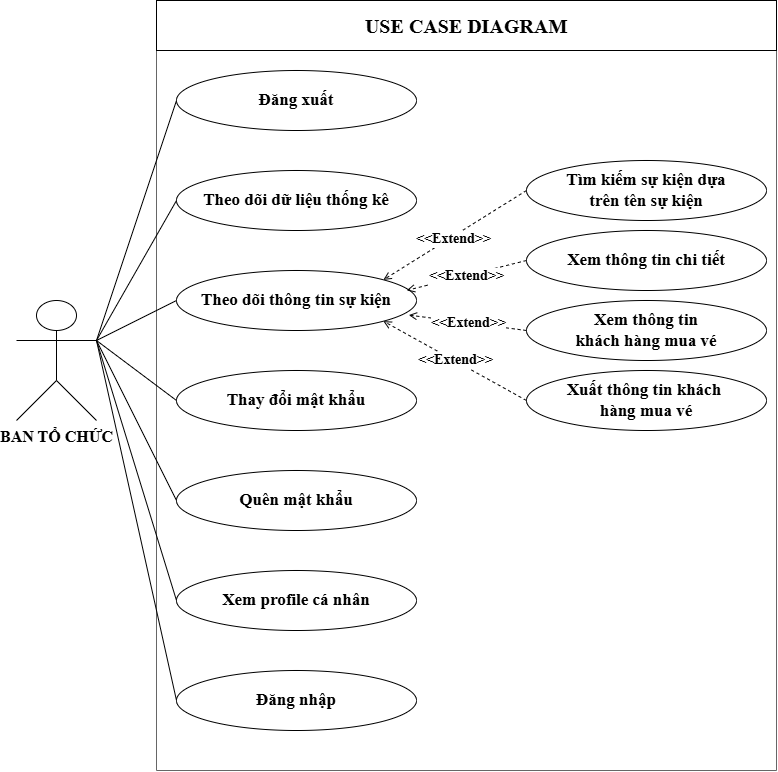
\includegraphics[width=1\textwidth]{Images/Ban tổ chức new.drawio.png}
    \vspace{10pt}
    \caption{Use Case Diagram -- Ban tổ chức}
    \label{fig:uc_organizer}
\end{figure}

\subsubsubsection{Đăng xuất}
\begin{table}[H]
\centering
\renewcommand{\arraystretch}{1.3}
\setlength{\tabcolsep}{8pt}
\begin{tabularx}{\textwidth}{|l|X|}
\hline
\textbf{Tên Use Case} & Đăng xuất \\ \hline
\textbf{Tác nhân} & Ban tổ chức \\ \hline
\textbf{Mục đích} & Cho phép Ban tổ chức đăng xuất khỏi hệ thống để bảo vệ tài khoản và thông tin cá nhân. \\ \hline        
\textbf{Điều kiện tiên quyết} & Ban tổ chức đã đăng nhập vào hệ thống. \\ \hline
\textbf{Điều kiện hậu quyết} & Ban tổ chức được đăng xuất thành công, phiên làm việc kết thúc và được chuyển hướng đến trang chủ hoặc trang đăng nhập. \\ \hline
\textbf{Mô tả ngắn gọn} & Ban tổ chức chọn chức năng đăng xuất để kết thúc phiên làm việc. \\ \hline
\textbf{Quy trình bình thường} &
1. Ban tổ chức nhấp vào nút “Đăng xuất” trên giao diện. \newline
2. Hệ thống xóa JWT token hoặc session liên quan đến phiên làm việc của Ban tổ chức. \newline
3. Hệ thống ghi log hoạt động đăng xuất. \newline
4. Hệ thống chuyển hướng Ban tổ chức đến trang chủ hoặc trang đăng nhập. \\ \hline
\textbf{Quy trình thay thế} &
2a. Nếu có lỗi khi xóa token/session: \newline
\hspace*{1em}- Hệ thống ghi log lỗi và vẫn chuyển hướng Ban tổ chức đến trang chủ hoặc trang đăng nhập để đảm bảo an toàn. \\ \hline
\textbf{Điều kiện lỗi} &
- Trường hợp lỗi 1: Lỗi hệ thống khi xử lý đăng xuất $\rightarrow$ Hệ thống ghi log lỗi và thông báo “Đăng xuất thất bại, vui lòng thử lại.” \newline
- Trường hợp lỗi 2: Lỗi kết nối khi ghi log $\rightarrow$ Hệ thống vẫn cho phép đăng xuất nhưng ghi log lỗi vào file cục bộ để kiểm tra sau. \\ \hline
\end{tabularx}
\vspace{15pt}
\caption{Đặc tả Use Case -- Đăng xuất (Ban tổ chức) }
\label{tab:uc_logout}
\end{table}

\subsubsubsection{Theo dõi dữ liệu thống kê}
\begin{table}[H]
\centering
\renewcommand{\arraystretch}{1.3}
\setlength{\tabcolsep}{8pt}
\begin{tabularx}{\textwidth}{|l|X|}
\hline
\textbf{Tên Use Case} & Theo dõi dữ liệu thống kê \\ \hline
\textbf{Tác nhân} & Ban tổ chức \\ \hline
\textbf{Mục đích} & Cho phép Ban tổ chức theo dõi các dữ liệu thống kê liên quan đến các sự kiện của mình tổ chức được đăng tải lên hệ thống \\ \hline
\textbf{Điều kiện tiên quyết} & Ban tổ chức đã đăng nhập vào hệ thống. \\ \hline
\textbf{Điều kiện hậu quyết} & Dữ liệu thống kê được hiển thị chính xác và cập nhật. \\ \hline
\textbf{Mô tả ngắn gọn} & Ban tổ chức truy cập vào mục thống kê để xem các số liệu thống kê liên quan đến các sự kiện của mình tổ chức. \\ \hline
\textbf{Quy trình bình thường} &
1. Ban tổ chức chọn mục “Statistical data” trên thanh sidebar. \newline
2. Hệ thống truy xuất dữ liệu liên quan đến sự kiện (Số sự kiện, Số vé đã đăng, Số vé đã bán, Tỉ lệ bán vé trung bình, Tổng doanh thu) từ cơ sở dữ liệu. \newline
3. Hệ thống hiển thị dữ liệu thống kê dưới dạng số liệu tổng quan. \\ \hline
\textbf{Quy trình thay thế} &
2a. Không có dữ liệu thống kê: Hệ thống hiển thị "Không có dữ liệu thống kê". \\ \hline
\textbf{Điều kiện lỗi} &
- Trường hợp lỗi 1: Lỗi kết nối cơ sở dữ liệu $\rightarrow$ Hệ thống hiển thị thông báo lỗi và ghi log để kiểm tra. \newline
- Trường hợp lỗi 2: Dữ liệu thống kê không chính xác $\rightarrow$ Hệ thống ghi log và thông báo “Data may be outdated, please refresh.” \\ \hline
\end{tabularx}
\vspace{15pt}
\caption{Đặc tả Use Case -- Theo dõi dữ liệu thống kê (Ban tổ chức) }
\label{tab:uc_statistics}
\end{table}


\subsubsubsection{Theo dõi thông tin sự kiện}

\begin{table}[H]
\centering
\renewcommand{\arraystretch}{1.3}
\setlength{\tabcolsep}{8pt}
\begin{tabularx}{\textwidth}{|l|X|}
\hline
\textbf{Tên Use Case} & Theo dõi thông tin sự kiện \\ \hline
\textbf{Tác nhân} & Ban tổ chức \\ \hline
\textbf{Mục đích} & 
Cho phép Ban tổ chức quản lý, tìm kiếm và theo dõi các thông tin chi tiết về sự kiện cùng danh sách khách hàng tham gia. \\ \hline
\textbf{Điều kiện tiên quyết} & 
- Ban tổ chức đã đăng nhập thành công vào hệ thống. \newline
- Ban tổ chức đã có các sự kiện được khởi tạo trên hệ thống. \\ \hline
\textbf{Điều kiện hậu quyết} & 
Thông tin chi tiết về sự kiện hoặc danh sách khách hàng được hiển thị/xuất file thành công. \\ \hline
\textbf{Mô tả ngắn gọn} & 
Ban tổ chức truy cập vào danh sách sự kiện để theo dõi trạng thái, xem chi tiết nội dung sự kiện hoặc quản lý danh sách khách hàng mua vé. \\ \hline
\textbf{Quy trình bình thường} &
1. Ban tổ chức chọn mục "Event Information" trên thanh sidebar. \newline
2. Hệ thống truy xuất và hiển thị danh sách các sự kiện do đơn vị này quản lý (bao gồm: poster, tên, thời gian, địa điểm, trạng thái). \newline
3. Ban tổ chức chọn xem thông tin chi tiết của một sự kiện cụ thể (icon Eye). \newline
4. Hệ thống hiển thị giao diện chi tiết nội dung sự kiện. \newline
5. Ban tổ chức chọn xem danh sách khách hàng mua vé (icon Person). \newline
6. Hệ thống hiển thị danh sách khách hàng tương ứng với sự kiện đã chọn. \newline
7. Ban tổ chức chọn đóng cửa sổ thông tin để quay lại danh sách sự kiện tổng quát. \\ \hline
\textbf{Quy trình thay thế} &
2a. Không có dữ liệu sự kiện: Hệ thống hiển thị thông báo "No data available". \newline
2b. Tìm kiếm sự kiện: Ban tổ chức nhập từ khóa, hệ thống lọc và hiển thị kết quả tương ứng. \newline
6a. Không có khách hàng mua vé: \newline
\hspace*{1em}- Hệ thống hiển thị danh sách trống và vô hiệu hóa (Không cho phép nhấn) các nút "Export CSV/PDF". \newline
\hspace*{1em}- Nếu người dùng cố gắng thực hiện lệnh xuất, hệ thống thông báo "No customer data to export". \newline
\textbf{6b. Xuất danh sách khách hàng:} \newline
\hspace*{1em}- Ban tổ chức chọn "Export CSV" hoặc "Export PDF". \newline
\hspace*{1em}- Hệ thống trích xuất dữ liệu và tải file xuống thiết bị. \\ \hline
\textbf{Điều kiện lỗi} &
- Lỗi kết nối: Hệ thống không thể kết nối Database, hiển thị thông báo lỗi hệ thống. \newline
- Lỗi trích xuất: Lỗi trong quá trình tạo file PDF/CSV, hệ thống thông báo "Export failed, please try again." \\ \hline
\end{tabularx}
\vspace{15pt}
\caption{Đặc tả Use Case -- Theo dõi thông tin sự kiện (Ban tổ chức)}
\label{tab:uc_view_search_event}
\end{table}

\subsubsubsection{Thay đổi mật khẩu}
\begin{table}[H]
\centering
\renewcommand{\arraystretch}{1.3}
\setlength{\tabcolsep}{8pt}
\begin{tabularx}{\textwidth}{|l|X|}
\hline
\textbf{Tên Use Case} & Thay đổi mật khẩu \\ \hline
\textbf{Tác nhân} & Ban tổ chức \\ \hline
\textbf{Mục đích} & Cho phép Ban tổ chức thay đổi mật khẩu để bảo vệ tài khoản. \\ \hline
\textbf{Điều kiện tiên quyết} & Ban tổ chức đã đăng nhập vào hệ thống. \\ \hline
\textbf{Điều kiện hậu quyết} & Mật khẩu được cập nhật thành công, Ban tổ chức nhận được thông báo popup. \\ \hline
\textbf{Mô tả ngắn gọn} & Ban tổ chức truy cập vào mục Đổi mật khẩu, nhập mật khẩu cũ và mật khẩu mới để cập nhật. \\ \hline
\textbf{Quy trình bình thường} &
1. Ban tổ chức chọn mục “Profile” trên thanh sidebar. \newline
2. Ban tổ chức chọn "Đổi mật khẩu". \newline
3. Hệ thống hiển thị form thay đổi mật khẩu (mật khẩu mới, xác nhận mật khẩu mới). \newline
4. Ban tổ chức nhập thông tin và gửi yêu cầu. \newline
5. Hệ thống xác thực tính hợp lệ của mật khẩu mới \newline
6. Nếu hợp lệ, hệ thống cập nhật mật khẩu mới vào cơ sở dữ liệu. \newline
7. Hệ thống ghi log hoạt động thay đổi mật khẩu. \newline
8. Hệ thống thông báo thành công và yêu cầu Ban tổ chức đăng nhập lại. \\ \hline
\textbf{Quy trình thay thế} &
% 4a. Mật khẩu cũ không chính xác $\rightarrow$ Hệ thống thông báo
% “Current password is incorrect” và yêu cầu nhập lại. \newline
5b. Mật khẩu mới không hợp lệ $\rightarrow$ Hệ thống thông báo lỗi và yêu cầu nhập lại. \newline
5c. Mật khẩu mới và xác nhận không khớp $\rightarrow$ Hệ thống thông báo “Mật khẩu mới không khớp” và yêu cầu nhập lại. \\ \hline
\textbf{Điều kiện lỗi} &    
- Trường hợp lỗi 1: Lỗi hệ thống khi cập nhật mật khẩu $\rightarrow$ Hệ thống ghi log lỗi và thông báo “Password change failed, please try again.” \newline
- Trường hợp lỗi 2: Lỗi kết nối khi ghi log $\rightarrow$ Hệ thống vẫn cho phép cập nhật mật khẩu nhưng ghi log lỗi vào file cục bộ để kiểm tra sau. \\ \hline
\end{tabularx}
\vspace{15pt}   
\caption{Đặc tả Use Case -- Thay đổi mật khẩu (Ban tổ chức) }
\label{tab:uc_change_password}
\end{table}

\subsubsubsection{Quên mật khẩu}
\begin{table}[H]
\centering
\renewcommand{\arraystretch}{1.3}
\setlength{\tabcolsep}{8pt}
\begin{tabularx}{\textwidth}{|l|X|} 
\hline
\textbf{Tên Use Case} & Quên mật khẩu \\ \hline
\textbf{Tác nhân} & Ban tổ chức \\ \hline
\textbf{Mục đích} & Cho phép Ban tổ chức khôi phục mật khẩu khi quên để tiếp tục sử dụng hệ thống. \\ \hline
\textbf{Điều kiện tiên quyết} & Ban tổ chức có tài khoản đã đăng ký trên hệ thống và có quyền truy cập email đã đăng ký. \\ \hline
\textbf{Điều kiện hậu quyết} & Ban tổ chức nhận được email cấp mật khẩu tạm thời, có thể đặt lại mật khẩu mới khi đăng nhập thành công. \\ \hline
\textbf{Mô tả ngắn gọn} & Ban tổ chức truy cập form đăng nhập, chọn “Quên mật khẩu”, nhập email để nhận hướng dẫn đặt lại mật khẩu. \\ \hline
\textbf{Quy trình bình thường} &   
1. Ban tổ chức truy cập form đăng nhập và chọn “Quên mật khẩu”. \newline
2. Hệ thống hiển thị form yêu cầu nhập email đã đăng ký. \newline
3. Ban tổ chức nhập email và gửi yêu cầu. \newline
4. Hệ thống xác thực email tồn tại trong cơ sở dữ liệu. \newline    
5. Nếu email hợp lệ, hệ thống tạo token khôi phục mật khẩu và gửi email có chứa mật khẩu mới tạm thời và hướng dẫn. \newline
6. Ban tổ chức nhận email. \newline
7. Ban tổ chức sử dụng mật khẩu tạm thời để đăng nhập thành công. \newline
8. Hệ thống sẽ điều hướng Ban tổ chức đến mục đặt lại mật khẩu mới. \newline
9. Ban tổ chức nhập mật khẩu mới và xác nhận, sau đó gửi yêu cầu. \newline
10. Hệ thống xác thực token và cập nhật mật khẩu mới vào cơ sở dữ liệu. \newline
11. Hệ thống ghi log hoạt động khôi phục mật khẩu. \newline
12. Hệ thống thông báo thành công \\ \hline
\textbf{Quy trình thay thế} &
4a. Email không tồn tại $\rightarrow$ Hệ thống thông báo lỗi và yêu cầu nhập lại. \newline
5b. Lỗi gửi email $\rightarrow$ Hệ thống ghi log lỗi và thông báo “Failed to send recovery email, please try again later.” \newline
8a. Token không hợp lệ hoặc hết hạn $\rightarrow$ Hệ thống thông báo “Invalid or expired token” và yêu cầu bắt đầu lại quy trình quên mật khẩu. \newline
8b. Mật khẩu mới không hợp lệ $\rightarrow$ Hệ thống thông báo lỗi và yêu cầu nhập lại. \newline
8c. Mật khẩu mới và xác nhận không khớp $\rightarrow$ Hệ thống thông báo “Mật khẩu mới không khớp” và yêu cầu nhập lại. \\ \hline
\textbf{Điều kiện lỗi} &    
- Trường hợp lỗi 1: Lỗi hệ thống khi cập nhật mật khẩu $\rightarrow$ Hệ thống ghi log lỗi và thông báo “Password reset failed, please try again.” \newline
- Trường hợp lỗi 2: Lỗi kết nối khi ghi log $\rightarrow$ Hệ thống vẫn cho phép đặt lại mật khẩu nhưng ghi log lỗi vào file cục bộ để kiểm tra sau. \\ \hline
\end{tabularx}
\vspace{15pt}
\caption{Đặc tả Use Case -- Quên mật khẩu (Ban tổ chức) }
\label{tab:uc_forgot_password}
\end{table}

\subsubsubsection{Xem profile cá nhân}
\begin{table}[H]
\centering
\renewcommand{\arraystretch}{1.3}
\setlength{\tabcolsep}{8pt}
\begin{tabularx}{\textwidth}{|l|X|}
\hline
\textbf{Tên Use Case} & Xem profile cá nhân \\ \hline
\textbf{Tác nhân} & Ban tổ chức \\ \hline
\textbf{Mục đích} & Cho phép Ban tổ chức xem thông tin cá nhân của mình. \\ \hline
\textbf{Điều kiện tiên quyết} & Ban tổ chức đã đăng nhập vào hệ thống. \\ \hline
\textbf{Điều kiện hậu quyết} & Thông tin cá nhân được hiển thị chính xác. \\ \hline
\textbf{Mô tả ngắn gọn} & Ban tổ chức truy cập vào mục Profile để xem thông tin cá nhân. \\ \hline
\textbf{Quy trình bình thường} &
1. Ban tổ chức chọn mục “Profile” trên thanh sidebar. \newline
2. Hệ thống truy xuất thông tin cá nhân (Name, Email, Phone, Address, Tax Code, Rating, Created At, Updated At) từ cơ sở dữ liệu. \newline
3. Hệ thống hiển thị thông tin cá nhân trên giao diện. \\ \hline
\textbf{Quy trình thay thế} &
2a. Không có dữ liệu cá nhân: Hệ thống hiển thị thông báo "No data". \\ \hline
\textbf{Điều kiện lỗi} &
- Trường hợp lỗi 1: Lỗi kết nối cơ sở dữ liệu $\rightarrow$ Hệ thống hiển thị thông báo lỗi và ghi log để kiểm tra. \newline
- Trường hợp lỗi 2: Dữ liệu cá nhân không tải được $\rightarrow$ Hệ thống ghi log và thông báo “Failed to load profile information, please try again.” \\ \hline
\end{tabularx}
\vspace{15pt}
\caption{Đặc tả Use Case -- Xem profile cá nhân (Ban tổ chức) }
\label{tab:uc_view_profile}
\end{table}


\subsubsection{Use Case cho Quản trị viên - OLD}
\begin{figure}[H]
    \centering
    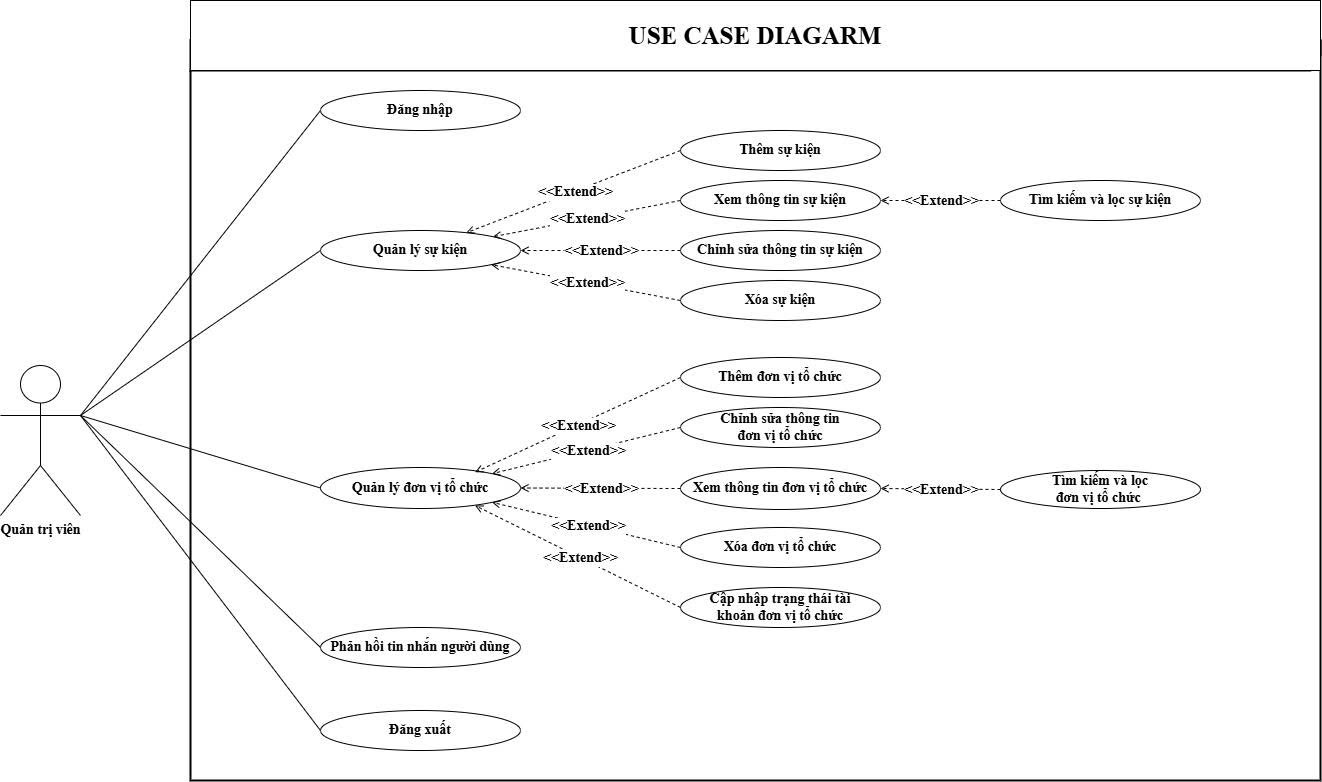
\includegraphics[width=1\textwidth]{Images/Usecase_Admin.jpg}
    \vspace{15pt}
    \caption{Use Case Diagram -- Quản trị viên}
    \label{fig:uc_admin}
\end{figure}

\subsubsubsection{Quản lý sự kiện}
\begin{table}[H]
\centering
\renewcommand{\arraystretch}{1.3}
\setlength{\tabcolsep}{8pt}
\begin{tabularx}{\textwidth}{|l|X|}
\hline
\textbf{Tên Use Case} & Quản lý sự kiện \\ \hline
\textbf{Tác nhân} & Admin \\ \hline
\textbf{Mục đích} & Quản lý thông tin sự kiện (thêm, sửa, xóa, tìm kiếm). \\ \hline
\textbf{Tiền điều kiện} & Admin đã đăng nhập. \\ \hline
\textbf{Hậu điều kiện} & Thông tin sự kiện được thêm mới, cập nhật hoặc xóa khỏi cơ sở dữ liệu. \\ \hline
\textbf{Luồng chính} &
1. Admin chọn chức năng “Quản lý sự kiện”. \newline
2. Hệ thống hiển thị danh sách sự kiện hiện có. \newline
3. Admin chọn thao tác: thêm, chỉnh sửa, xóa hoặc xem chi tiết sự kiện. \newline
4. Hệ thống xử lý yêu cầu và cập nhật dữ liệu. \\ \hline
\textbf{Luồng thay thế} &
3a. Nếu Admin chọn “Tìm kiếm/Lọc sự kiện”: \newline
\hspace*{1em}a. Hệ thống hiển thị ô tìm kiếm. \newline
\hspace*{1em}b. Admin nhập từ khóa $\to$ Hệ thống hiển thị danh sách kết quả phù hợp. \\ \hline
\textbf{Điều kiện lỗi} &
1. Nhập thiếu thông tin bắt buộc khi thêm sự kiện $\to$ Hệ thống báo lỗi và yêu cầu nhập lại. \newline
2. Lỗi hệ thống khi ghi dữ liệu $\to$ Hệ thống hiển thị thông báo thất bại. \\ \hline
\end{tabularx}
\vspace{15pt}
\caption{Đặc tả Use Case -- Quản lý sự kiện}
\label{tab:uc_manage_event}
\end{table}

\subsubsubsection{Quản lý đơn vị tổ chức}

\begin{table}[H]
\centering
\renewcommand{\arraystretch}{1.3}
\setlength{\tabcolsep}{8pt}
\begin{tabularx}{\textwidth}{|l|X|}
\hline
\textbf{Tên Use Case} & Quản lý đơn vị tổ chức \\ \hline
\textbf{Tác nhân} & Admin \\ \hline
\textbf{Mục đích} & Quản lý thông tin đơn vị tổ chức (thêm, sửa, xóa, tìm kiếm). \\ \hline
\textbf{Tiền điều kiện} & Admin đã đăng nhập. \\ \hline
\textbf{Hậu điều kiện} & Thông tin đơn vị tổ chức được thêm, cập nhật hoặc xóa khỏi hệ thống. \\ \hline
\textbf{Luồng chính} &
1. Admin truy cập chức năng “Quản lý đơn vị tổ chức”. \newline
2. Hệ thống hiển thị danh sách đơn vị. \newline
3. Admin chọn thao tác: thêm, chỉnh sửa, xóa hoặc xem chi tiết đơn vị. \newline
4. Hệ thống xử lý và lưu kết quả vào cơ sở dữ liệu. \\ \hline
\textbf{Luồng thay thế} &
3a. Nếu Admin chọn “Tìm kiếm/Lọc đơn vị”: \newline
\hspace*{1em}a. Hệ thống hiển thị ô tìm kiếm. \newline
\hspace*{1em}b. Admin nhập từ khóa $\rightarrow$ Hệ thống hiển thị danh sách kết quả phù hợp. \newline
3b. Nếu Admin chọn “Cập nhật trạng thái đơn vị”: \newline
\hspace*{1em}a. Hệ thống hiển thị danh sách trạng thái mới. \newline
\hspace*{1em}b. Admin chọn và lưu thay đổi. \\ \hline
\textbf{Điều kiện lỗi} &
1. Nhập thiếu thông tin bắt buộc khi thêm đơn vị $\rightarrow$ Hệ thống báo lỗi và yêu cầu nhập lại. \newline
2. Lỗi hệ thống khi ghi dữ liệu $\rightarrow$ Hệ thống hiển thị thông báo thất bại. \\ \hline
\end{tabularx}
\vspace{15pt}
\caption{Đặc tả Use Case -- Quản lý đơn vị tổ chức}
\label{tab:uc_manage_organizer}
\end{table}

% %%%%%%%%%%%%%% Activity diagram


\subsection{Lược đồ hoạt động}

\subsubsection{Activity Diagram cho Người dùng - OLD}

\subsubsubsection{Đăng ký}
\begin{figure}[H]
    \centering
    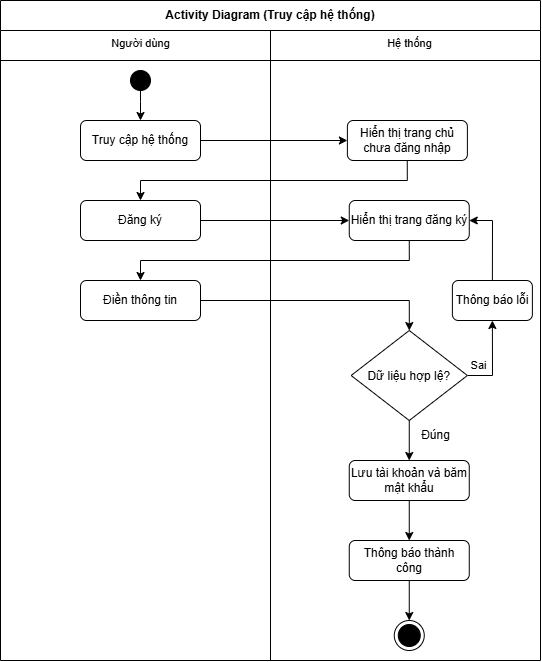
\includegraphics[width=0.7\textwidth]{Images/DangKy_ActivityDiagram.png}
    \vspace{15pt}
    \caption{Activity Diagram -- Đăng ký tài khoản}
\end{figure}

\indent \indent Người dùng chọn đăng kí tài khoản nếu chưa có tài khoản. Người dùng sẽ được chuyển hướng tới trang đăng kí. Sau khi người dùng nhập thông tin và chọn đăng kí, nếu
thông tin đã nhập là hợp lệ thì hệ thống sẽ lưu tài khoản và mã hóa mật khẩu. Trường hợp thông tin đã nhập được xác định là chưa hợp lệ, người dùng buộc phải nhập lại.


\subsubsubsection{Đăng nhập}
\begin{figure}[H]
    \centering
    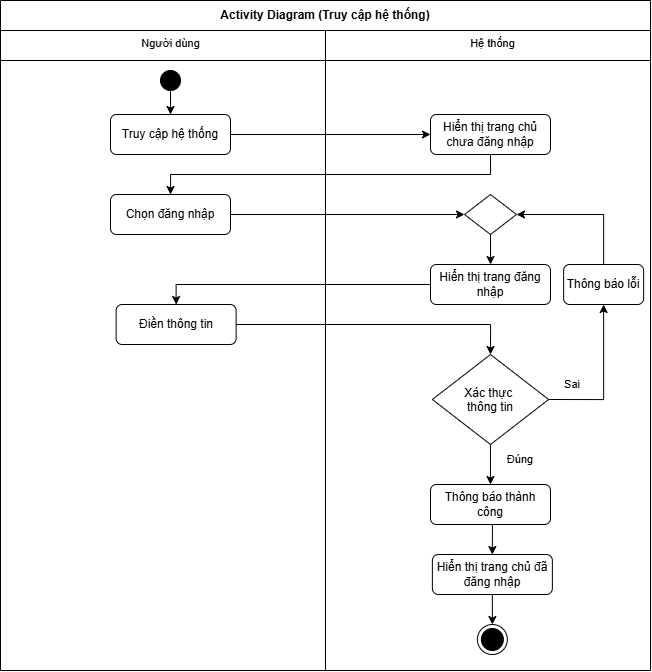
\includegraphics[width=0.7\textwidth]{Images/DangNhap_ActivityDiagram.png}
    \vspace{15pt}
    \caption{Activity Diagram -- Đăng nhập tài khoản}
\end{figure}

\indent \indent Người dùng sẽ nhập thông tin tài khoản để đăng nhập vào hệ thống. Sau khi đăng nhập thành công thì hệ thống sẽ chuyển hướng đến trang chủ. \\
\indent \underline{Lưu ý:} Sơ đồ hoạt động đăng nhập tài khoản trên có thể áp dụng cho cả Ban tổ chức hoặc quản trị viên trong cùng hoạt động.

\subsubsubsection{Mua vé sự kiện}

\begin{figure}[H]
    \centering
    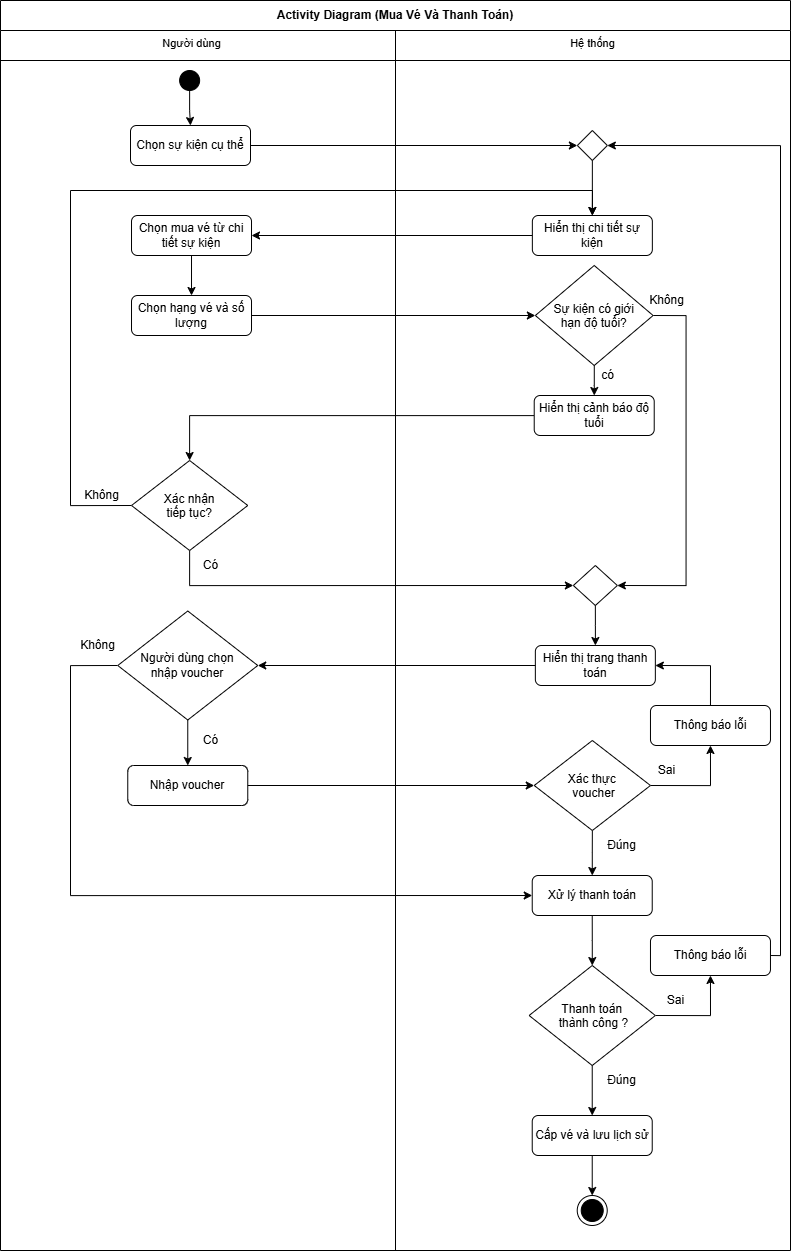
\includegraphics[width=0.7\textwidth]{Images/MuaVe_ActivityDiagram.png}
    \vspace{15pt}
    \caption{Activity Diagram -- Mua vé sự kiện}
\end{figure}

\subsubsubsection{Chat với Ban tổ chức hoặc quản trị viên}

\subsubsection{Activity Diagram cho Ban tổ chức}

\subsubsubsection{Theo dõi dữ liệu thống kê}
\begin{figure}[H]
    \centering
    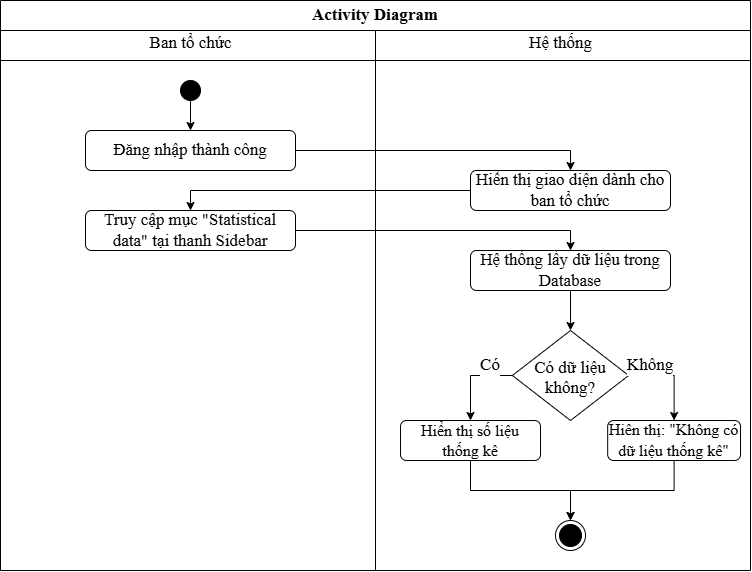
\includegraphics[width=0.7\textwidth]{Images/Activity_Diagram_BTC/Ativity Diagram-Xem dữ liệu thống kê.drawio.png}
    \vspace{15pt}
    \caption{Activity Diagram -- Theo dõi dữ liệu thống kê (Ban tổ chức)}
\end{figure}

\indent \indent Ban tổ chức sẽ truy cập vào mục Statistical data trên thanh Sidebar để theo dõi các số liệu thống kê liên quan đến các sự kiện của mình tổ chức được đăng tải lên hệ thống. Hệ thống sẽ truy xuất dữ liệu liên quan đến sự kiện (Số sự kiện, Số vé đã đăng, Số vé đã bán, Tỉ lệ bán vé trung bình, Tổng doanh thu) từ cơ sở dữ liệu và hiển thị dữ liệu thống kê dưới dạng số liệu tổng quan. Nếu có lỗi kết nối cơ sở dữ liệu hoặc dữ liệu thống kê không chính xác, hệ thống có thông báo lỗi và hiển thị "Không có dữ liệu thống kê".

\subsubsubsection{Theo dõi thông tin sự kiện}
\begin{figure}[H]
    \centering
    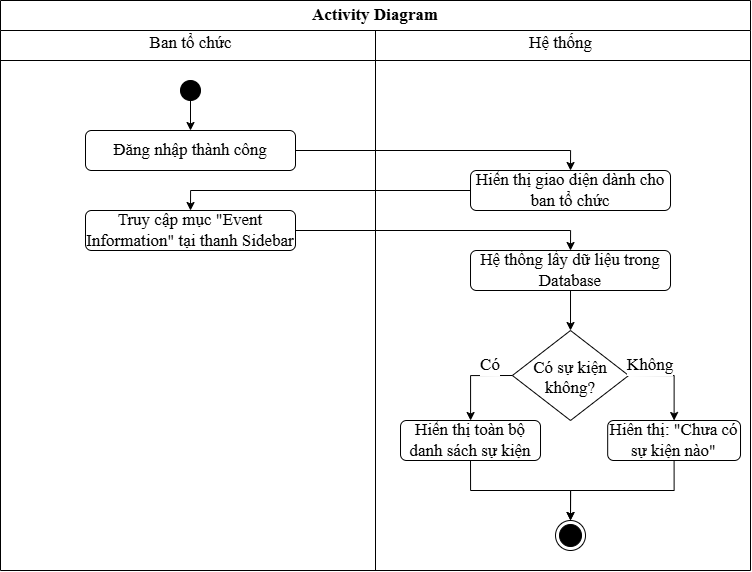
\includegraphics[width=0.7\textwidth]{Images/Activity_Diagram_BTC/Ativity Diagram-Xem danh sách sự kiện.drawio.png}
    \vspace{15pt}
    \caption{Activity Diagram -- Theo dõi thông tin sự kiện (Ban tổ chức)}
\end{figure}

\indent \indent Ban tổ chức sẽ truy cập vào mục Event Information trên thanh Sidebar để xem danh sách các sự kiện do mình tổ chức. Hệ thống sẽ truy xuất và hiển thị danh sách các sự kiện, bao gồm poster, tên, thời gian, địa điểm và trạng thái. \\
\indent Tại giao diện danh sách sự kiện tổng quan, Ban tổ chức có thể nhập từ khóa vào thanh tìm kiếm để lọc các sự kiện. Nếu có lỗi kết nối cơ sở dữ liệu hoặc không có dữ liệu sự kiện phù hợp, hệ thống sẽ hiển thị thông báo lỗi và hiển thị "No data".
\begin{figure}[H]
    \centering
    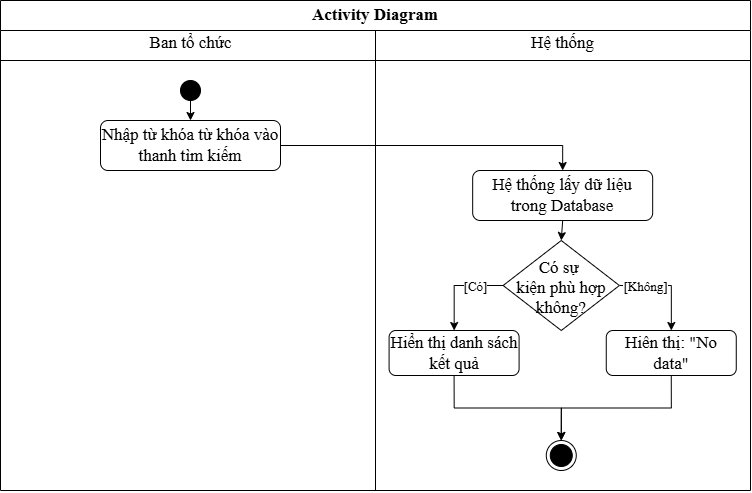
\includegraphics[width=0.7\textwidth]{Images/Activity_Diagram_BTC/Ativity Diagram-Tìm kiếm sự kiện.drawio.png}
    \vspace{15pt}
    \caption{Activity Diagram -- Tìm kiếm sự kiện (Ban tổ chức)}
\end{figure}

\indent Để xem thông tin chi tiết của một sự kiện cụ thể, Ban tổ chức sẽ chọn icon Eye tương ứng với sự kiện đó ở cột Action. Hệ thống sẽ hiển thị giao diện bảng chi tiết nội dung sự kiện. Để tắt giao diện bảng thông tin chi tiết, Ban tổ chức cần nhấn dấu X ở góc phải và giao diện sẽ quay về giao diện danh sách dữ liệu tổng quan ban đầu \\
\begin{figure}
    \centering
    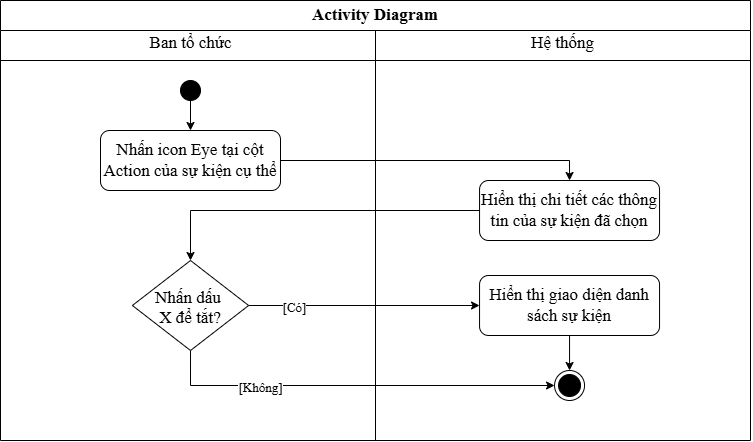
\includegraphics[width=0.7\textwidth]{Images/Activity_Diagram_BTC/Ativity Diagram-xem chi tiết thông tin sự kiện.drawio.png}
    \vspace{15pt}
    \caption{Activity Diagram -- Xem chi tiết sự kiện (Ban tổ chức)}
\end{figure}

\indent Ban tổ chức cũng có thể chọn icon Person tương ứng với sự kiện đó ở cột Action để xem danh sách khách hàng đã mua vé cho sự kiện đó. Hệ thống sẽ hiển thị giao diện bảng danh sách khách hàng mua vé tương ứng với sự kiện đã chọn. Ban tổ chức có thể nhấn vào một trong hai nút xuất file dữ liệu khách hàng trên về máy với định dạng CSV hoặc PDF.
Nếu có lỗi kết nối cơ sở dữ liệu hoặc không có dữ liệu về các khách hàng đã mua vé, hệ thống sẽ có thông báo lỗi, hiển thị danh sách khách hàng trống và vô hiệu hóa các nút xuất file dữ liệu khách hàng.
\begin{figure}
    \centering
    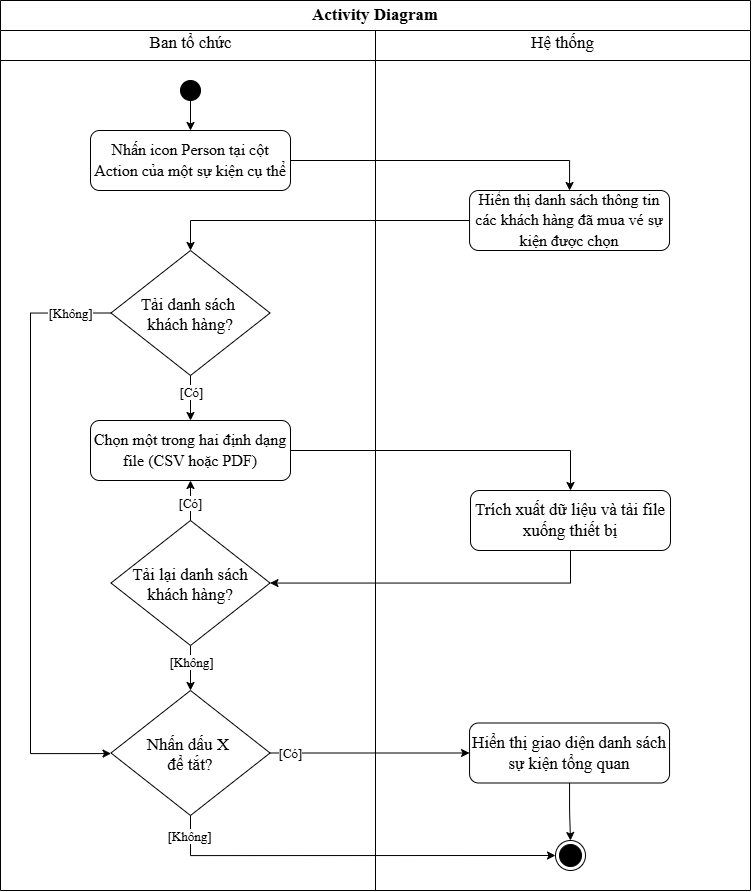
\includegraphics[width=0.7\textwidth]{Images/Activity_Diagram_BTC/Ativity Diagram-Xem_xuất thông tin khách hàng đã mua vé 1 sự kiện cụ thể.drawio.png}
    \vspace{15pt}
    \caption{Activity Diagram -- Xem danh sách khách hàng mua vé (Ban tổ chức)}
\end{figure}

\subsubsubsection{Thay đổi mật khẩu}
\begin{figure}[H]
    \centering
    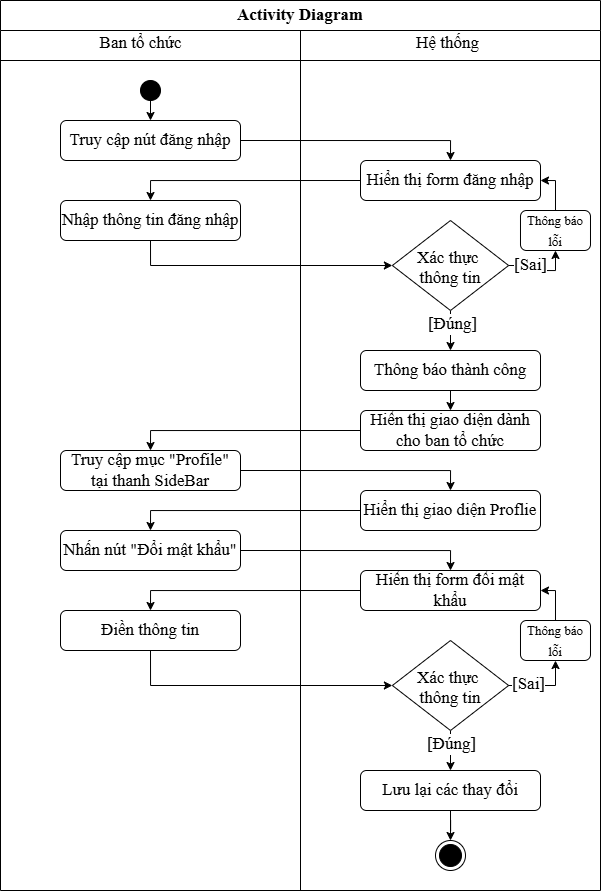
\includegraphics[width=0.7\textwidth]{Images/Activity_Diagram_BTC/Ativity Diagram-Đổi mật khẩu.drawio.png}
    \vspace{15pt}
    \caption{Activity Diagram -- Thay đổi mật khẩu (Ban tổ chức)}
\end{figure}

\indent \indent Khi có nhu cầu đổi mật khẩu, Ban tổ chức sẽ truy cập vào mục Profile tại thanh Sidebar và chọn chức năng đổi mật khẩu. Hệ thống sẽ hiển thị form yêu cầu nhập mật khẩu mới và xác nhận mật khẩu mới. Ban tổ chức nhập thông tin và gửi yêu cầu. Hệ thống sẽ kiểm tra tính hợp lệ của mật khẩu mới, nếu hợp lệ thì cập nhật mật khẩu mới vào cơ sở dữ liệu, ghi log hoạt động và thông báo thành công. Nếu có lỗi hoặc thông tin không hợp lệ, hệ thống sẽ thông báo lỗi và yêu cầu nhập lại.

\subsubsubsection{Quên mật khẩu}
\begin{figure}[H]
    \centering
    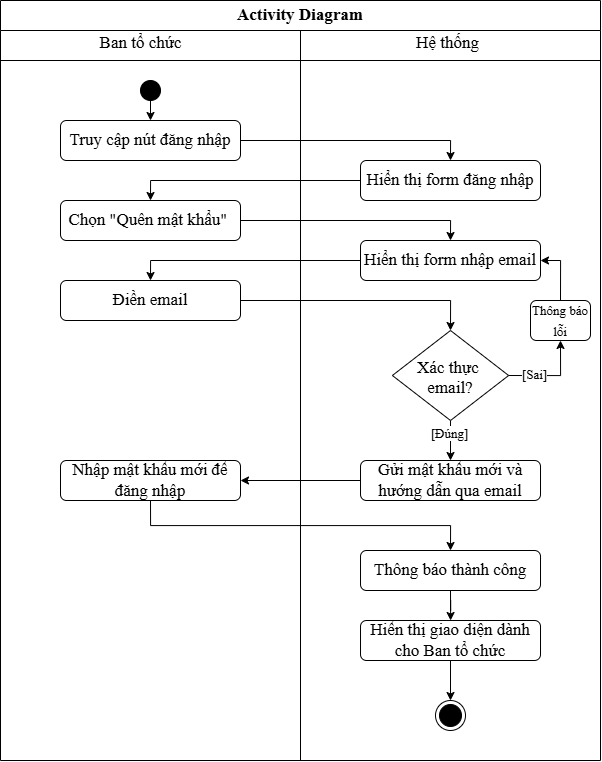
\includegraphics[width=0.7\textwidth]{Images/Activity_Diagram_BTC/Ativity Diagram-Quên mật khẩu.drawio.png}
    \vspace{15pt}
    \caption{Activity Diagram -- Quên mật khẩu (Ban tổ chức)}
\end{figure}

\indent \indent Khi quên mật khẩu, Ban tổ chức sẽ truy cập vào form đăng nhập và chọn chức năng quên mật khẩu. Hệ thống sẽ hiển thị form yêu cầu nhập email đã đăng ký. Ban tổ chức nhập email và gửi yêu cầu. Hệ thống sẽ xác thực xem email có định dạng hợp lệ và có tài khoản nào được tạo với email trên hay không, nếu đáp ứng cả hai yêu cầu thì tạo token khôi phục mật khẩu và gửi mật khẩu mới tạm thời kèm hướng dẫn qua email trên. Ban tổ chức nhận email, sử dụng mật khẩu tạm thời để đăng nhập thành công và được hệ thống điều hướng tự động tới mục đổi mật khẩu. Ban tổ chức sẽ thực hiện quy trình đổi sang mật khẩu mới như được mô tả ở \textbf{mục 5.2.2.c}. Hệ thống sẽ xác thực token, cập nhật mật khẩu mới vào cơ sở dữ liệu, ghi log hoạt động và thông báo thành công. Nếu có lỗi hoặc thông tin không hợp lệ, hệ thống sẽ thông báo lỗi và yêu cầu nhập lại.

\subsubsubsection{Xem profile cá nhân}

\begin{figure}[H]
    \centering
    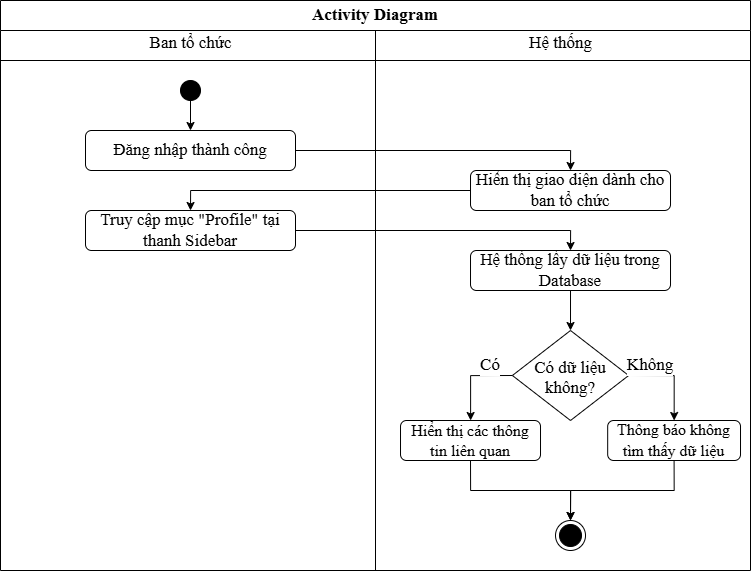
\includegraphics[width=0.7\textwidth]{Images/Activity_Diagram_BTC/Ativity Diagram-Profile.drawio.png}
    \vspace{15pt}
    \caption{Activity Diagram -- Xem profile cá nhân (Ban tổ chức)}
\end{figure}

\indent \indent Ban tổ chức có thể xem thông tin cá nhân của mình, bao gồm  Name, Email, Phone, Address, Tax Code, Rating, Created At và Updated At. Hệ thống sẽ hiển thị các thông tin này khi Ban tổ chức truy cập vào mục Profile trên thanh Sidebar. Nếu có lỗi khi tải thông tin cá nhân, hệ thống sẽ hiển thị thông báo lỗi và giá trị ở các trường sẽ hiển thị là "--". 

\subsubsection{Activity Diagram cho Quản trị viên - OLD}

\subsubsubsection{Quản lý danh sách các sự kiện}
\begin{figure}[H]
    \centering
    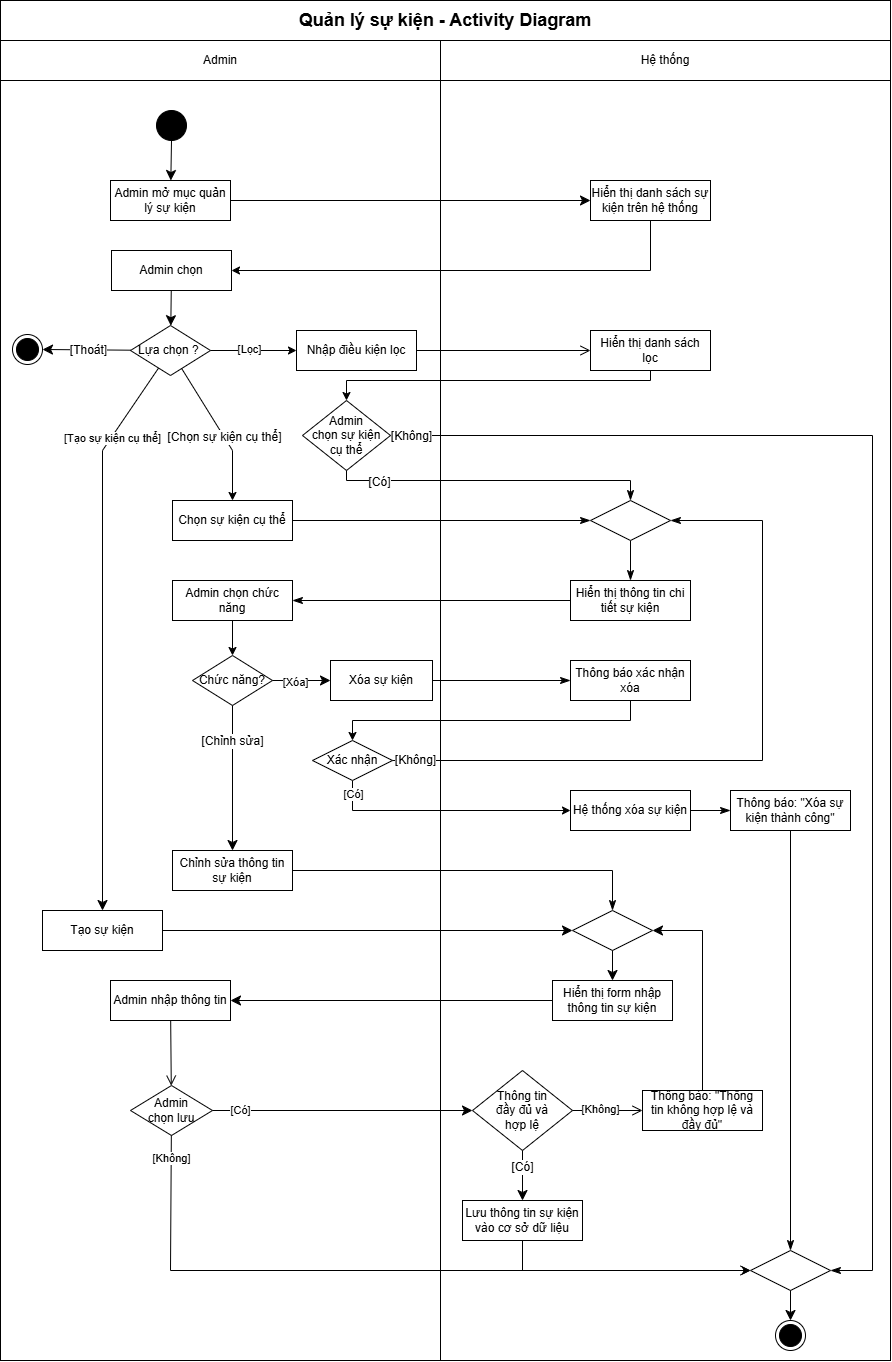
\includegraphics[width=0.7\textwidth]{Images/QuanLySuKien_ActivityDiagram.png}
    \vspace{15pt}
    \caption{Activity Diagram -- Quản lý danh sách sự kiện}
\end{figure}
\indent \indent Đầu tiên, admin mở mục quản lý sự kiện và có thể lọc hoặc chọn một sự kiện cụ thể để xem chi tiết. Từ đây, admin có thể thực hiện các chức năng như tạo mới, chỉnh sửa hoặc xóa sự kiện. Nếu xóa, hệ thống sẽ yêu cầu xác nhận và hiển thị thông báo sau khi xóa thành công; nếu chỉnh sửa hoặc tạo mới, hệ thống hiển thị form nhập liệu để admin điền thông tin. Sau khi admin lưu, hệ thống kiểm tra tính hợp lệ và đầy đủ của dữ liệu, rồi lưu thông tin vào cơ sở dữ liệu và thông báo kết quả tương ứng.
\subsubsubsection{Quản lý đơn vị tổ chức sự kiện}
\begin{figure}[H]
    \centering
    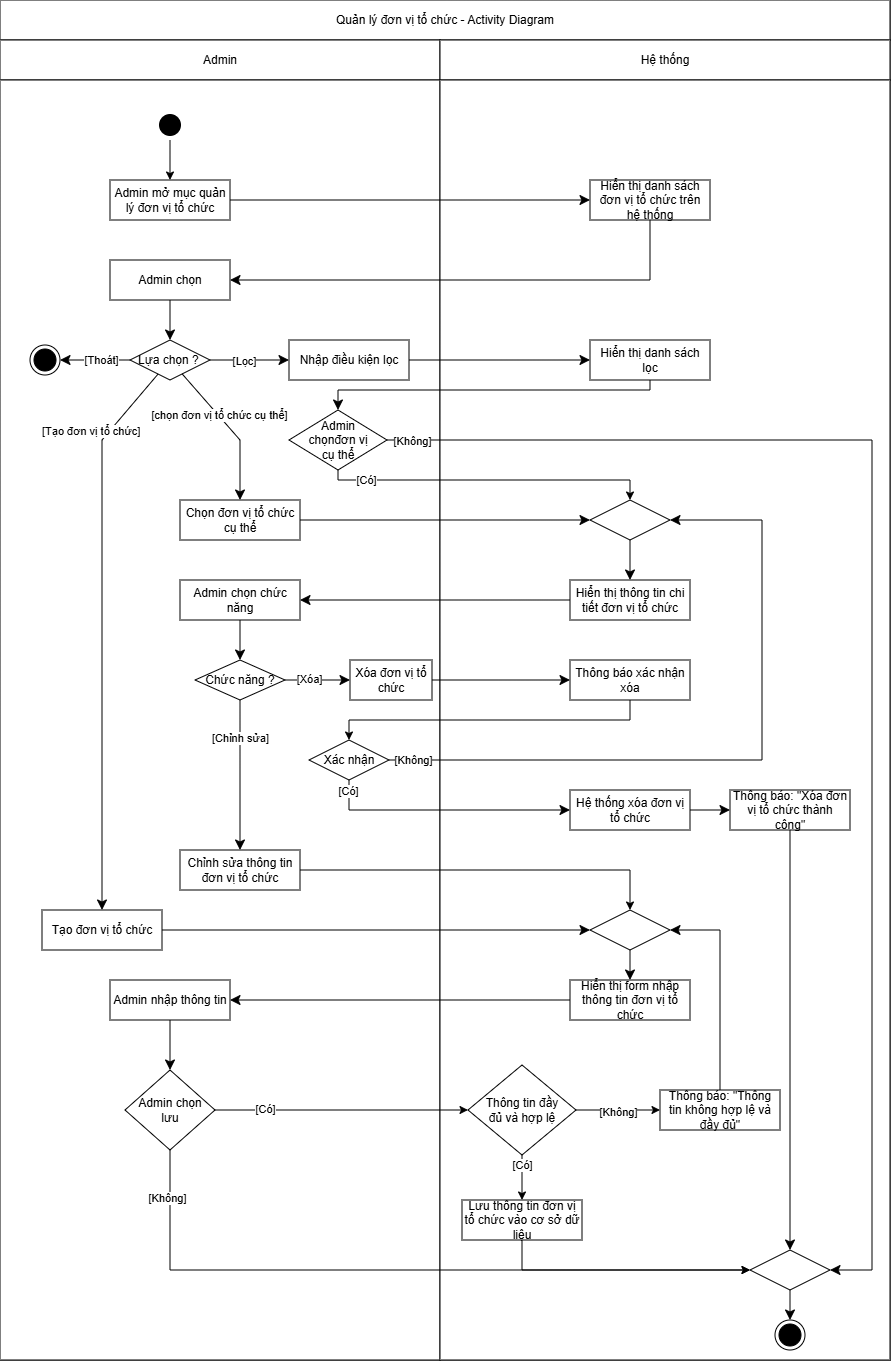
\includegraphics[width=0.7\textwidth]{Images/QuanLyToChuc_ActivityDiagram.png}
    \vspace{15pt}
    \caption{Activity Diagram -- Quản lý các đơn vị tổ chức sự kiện}
\end{figure}
\indent \indent Đầu tiên, admin truy cập mục quản lý và có thể thực hiện lọc danh sách hoặc chọn đơn vị cụ thể để xem chi tiết. Sau đó, admin có thể thực hiện các chức năng như tạo mới, chỉnh sửa hoặc xóa đơn vị tổ chức. Khi thực hiện thao tác xóa, hệ thống sẽ yêu cầu xác nhận trước khi xóa dữ liệu. Đối với thao tác thêm hoặc chỉnh sửa, hệ thống kiểm tra tính hợp lệ của thông tin và lưu vào cơ sở dữ liệu nếu hợp lệ, đồng thời hiển thị thông báo kết quả tương ứng.


%%%%%%%%%%%% Sequence diagram

\subsection{Lược đồ tuần tự - OLD}

\subsubsection{Chức năng mua vé dành cho người dùng}

\begin{figure}[H]
    \centering
    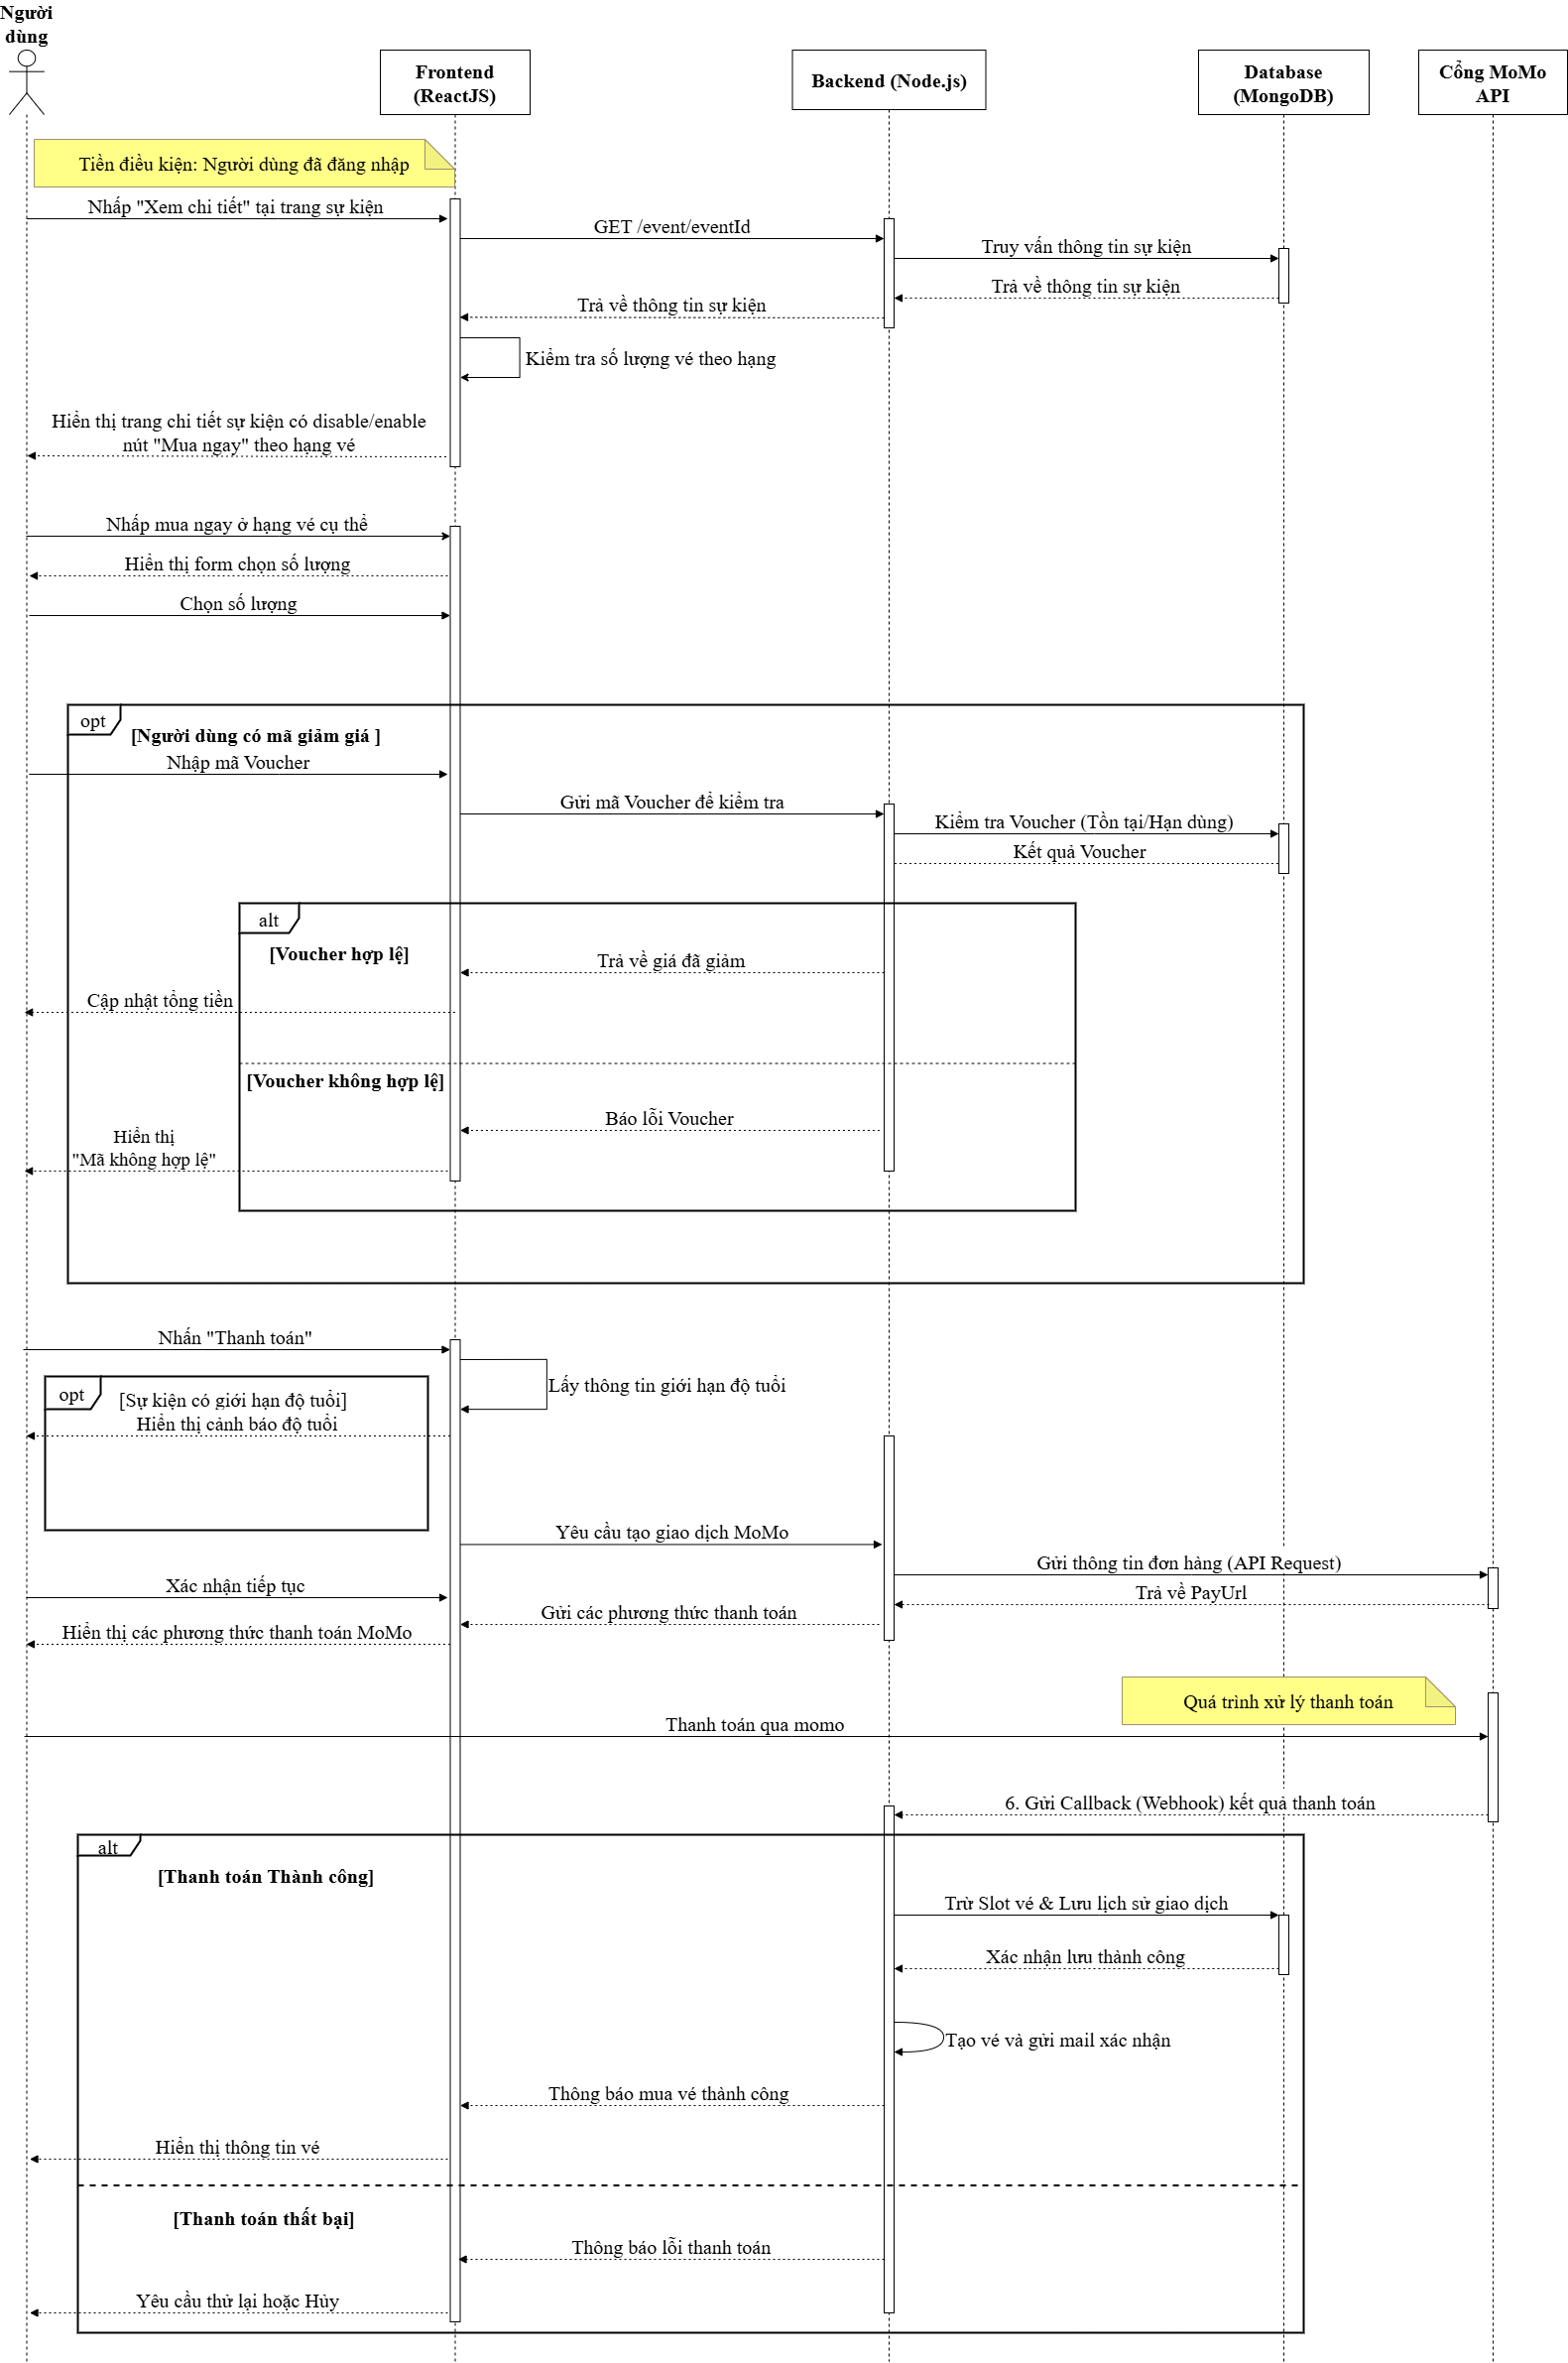
\includegraphics[width=0.9\textwidth]{Images/seq_muave.png}
    \vspace{15pt}
    \caption{Sequence Diagram -- Chức năng mua vé dành cho người dùng}
\end{figure}

\subsubsection{Chức năng gợi ý sự kiện cá nhân hóa dành cho người dùng}

\begin{figure}[H]
    \centering
    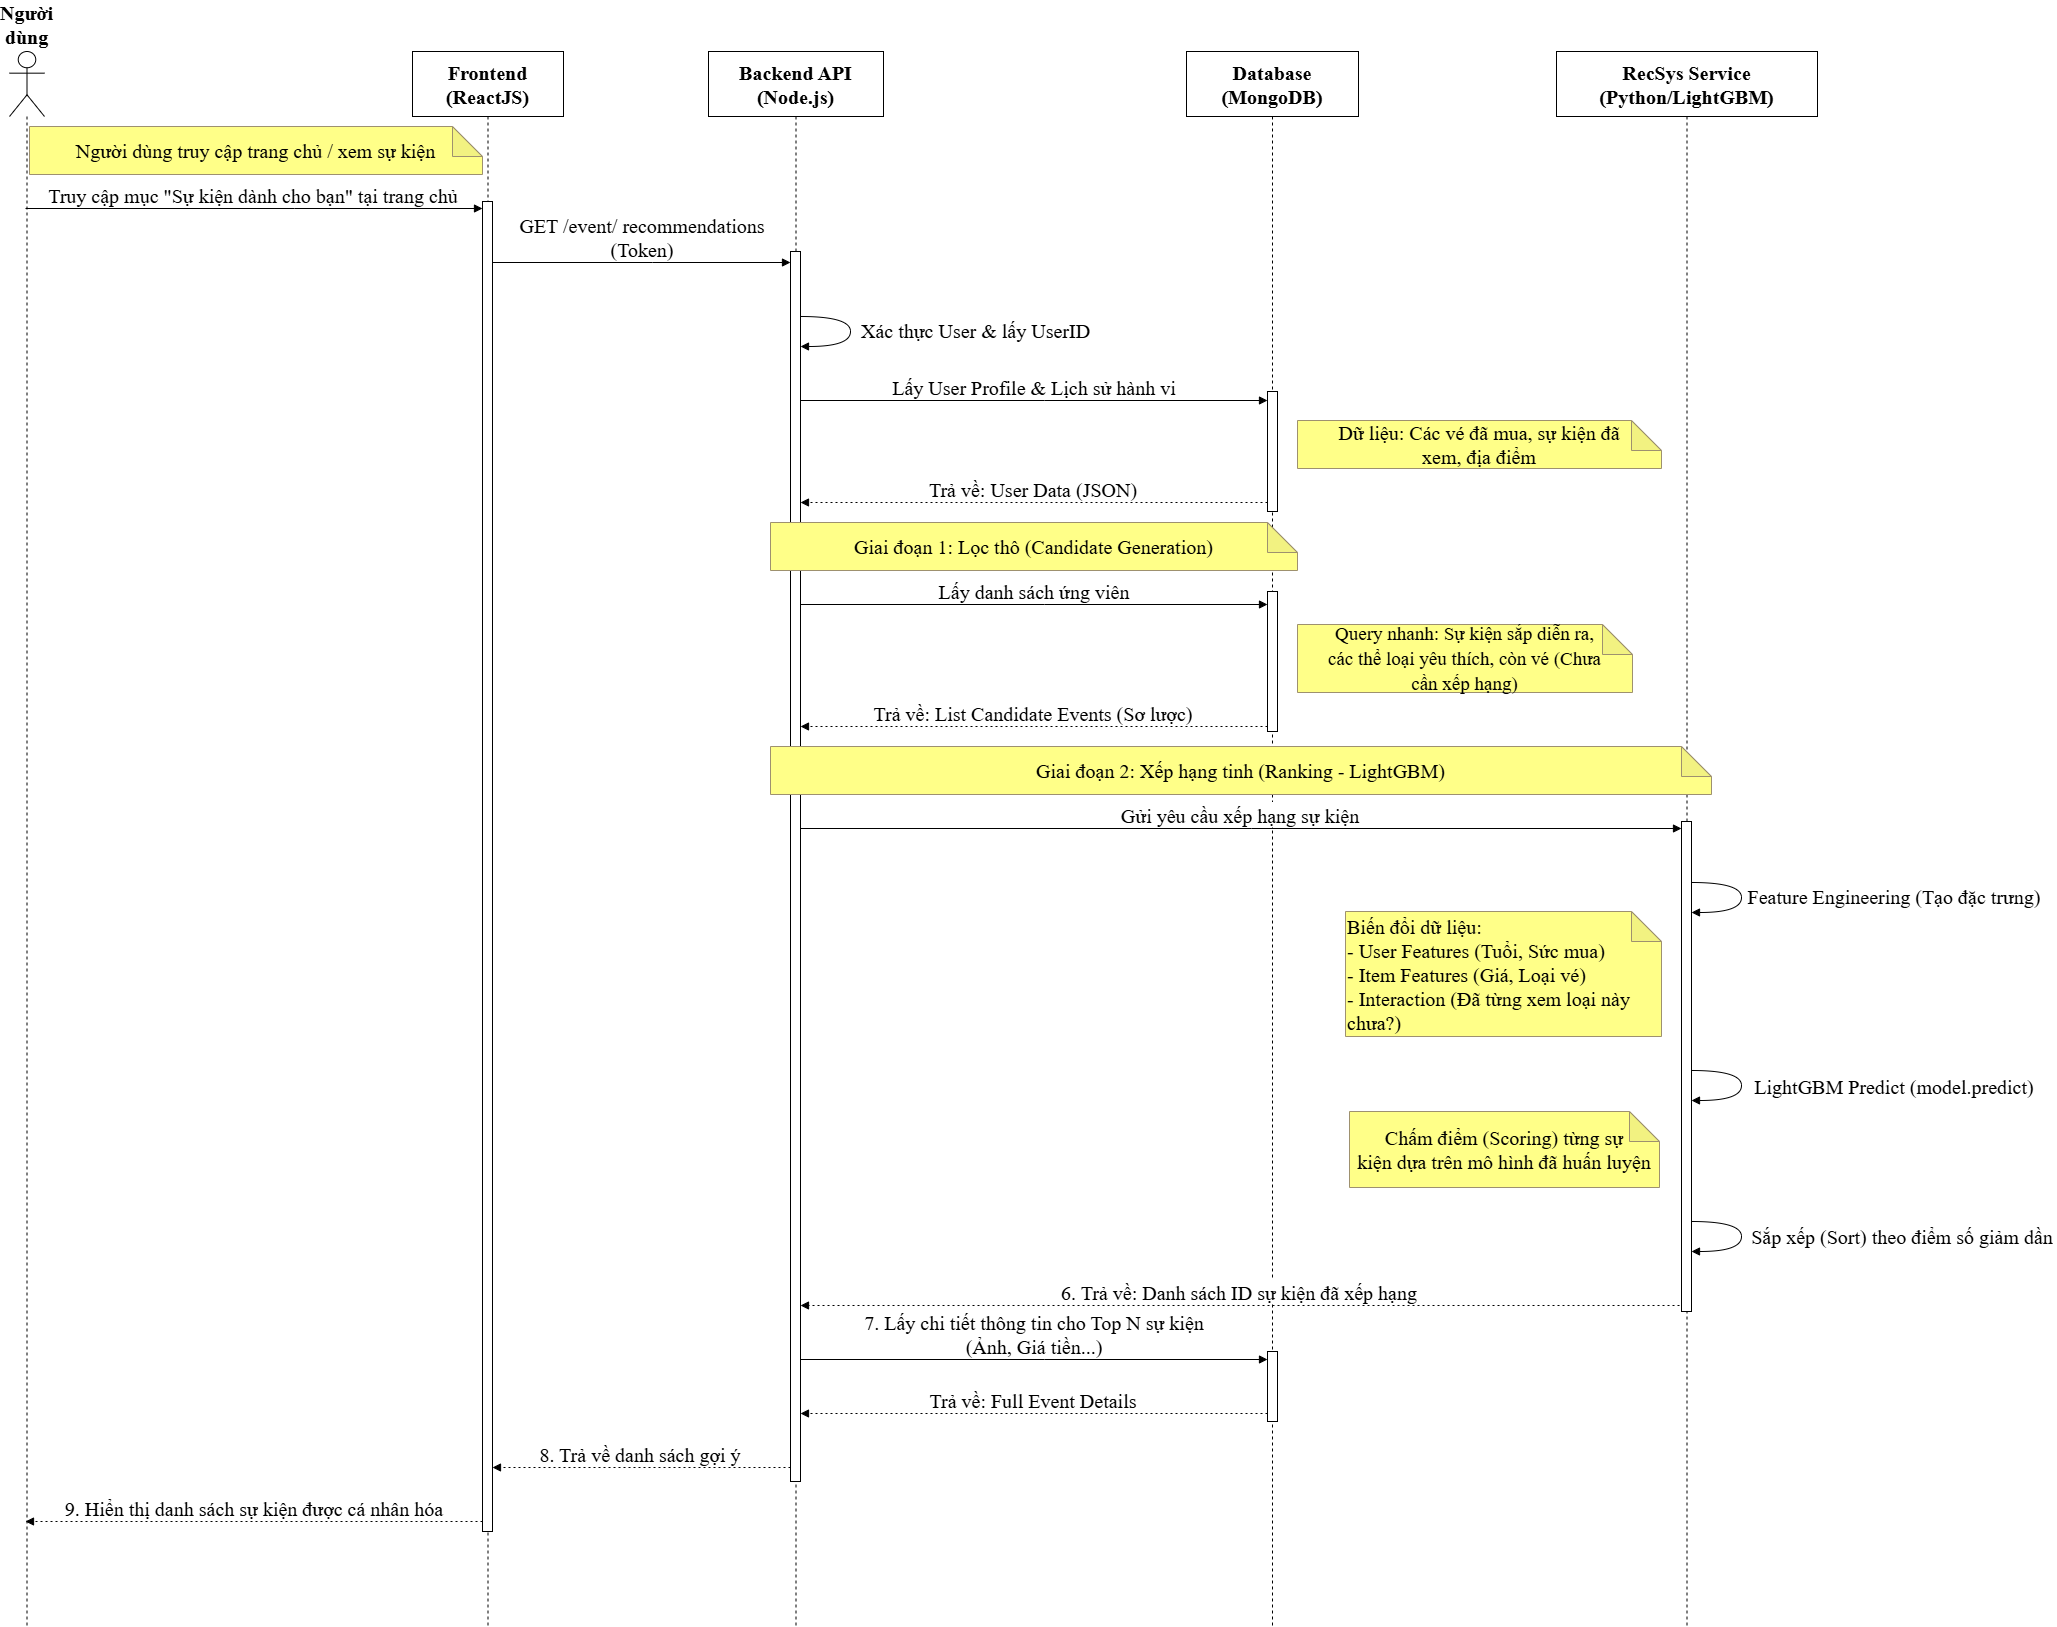
\includegraphics[width=1\textwidth]{Images/seq_goiy.png}
    \vspace{15pt}
    \caption{Sequence Diagram -- Chức năng gợi ý sự kiện cá nhân hóa dành cho người dùng}
\end{figure}

\subsubsection{Chức năng nhắn tin}

\begin{figure}[H]
    \centering
    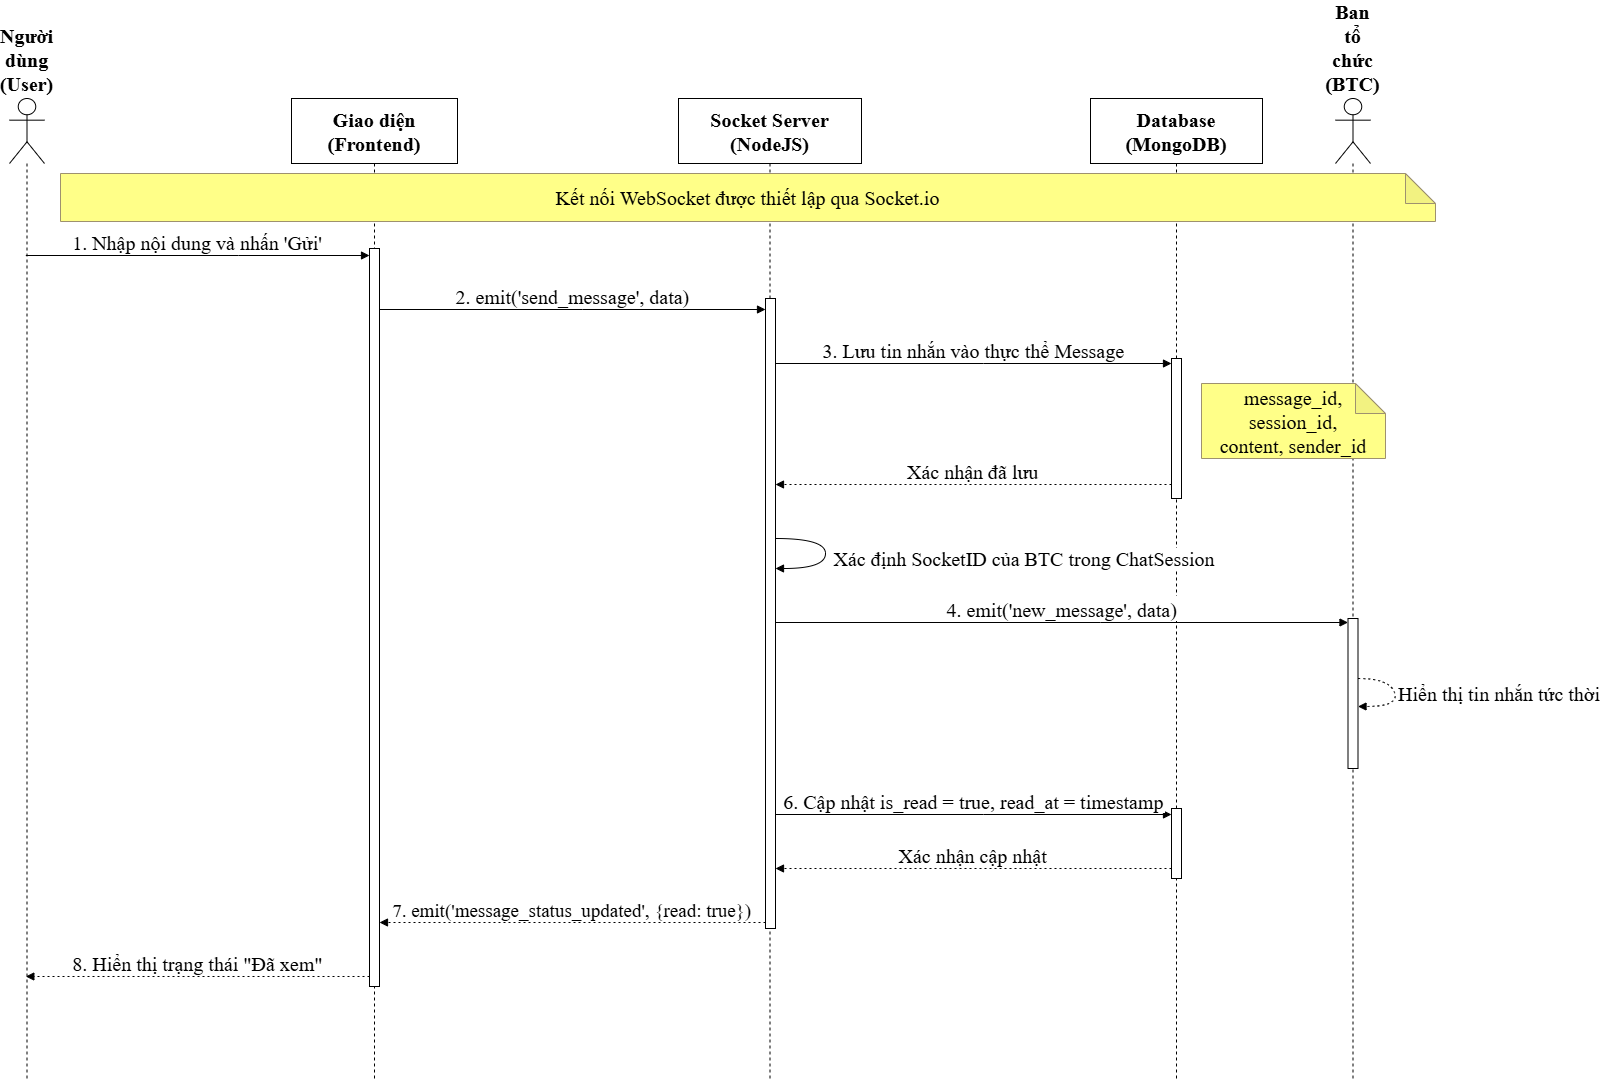
\includegraphics[width=1\textwidth]{Images/seq_chat.png}
    \vspace{15pt}
    \caption{Sequence Diagram -- Chức năng nhắn tin}
\end{figure}
